% !TEX root = ./../main.tex
\chapter{Molecular description of the process}
%Introduzione a seguito dei risultati con la metadinamica: run unbiased con PW striped, random11, random 12 e POPC
In view of the results obtained with metadynamics, shown in the previous chapter, and in order to try to see the anchoring process to spontaneously occur, we decide to perform unbiased runs starting from the hydrophobic state for all the anionic \ac{AuNP} configurations: the striped (\ac{MUS}:\ac{OT} $1$:$1$), the random (\ac{MUS}:\ac{OT} $1$:$1$) and the random (\ac{MUS}:\ac{OT} $2$:$1$), with both \ac{PME} and \ac{PW} model. This runs are suitable to get some useful information about the molecular processes involved and about the hydrophobic state with a more realistic \ac{CG} description.

Unfortunately, with ten of microseconds for each configurations, we have not seen any anchoring process. This confirm, in accordance with the atomistic model and the metadynamics results, the increase of the energy barrier respect to the standard \martini model and the slowdown of the dynamics of the system. Despite this, the unbiased runs are useful in order for a comparison with the metadynamics runs to be made. In particular we can compare some interesting molecular phenomena that we have see in metadynamics runs such as: the water bead dragging inside the hydrophobic region of the membrane by the charged bead during the anchoring process; the choline group bead of the entrance leaflet dragging inside the hydrophobic region by the charged bead during the anchoring process and the engulfment effect of the opposite leaflet during the dis--anchor process. Moreover, comparing the results of the hydrophobic state only, we can get some information about the destructiveness of the metadynamics and if and how the bilayer properties change. 


\section{Water dragging}
%Trascinamento delle PW nelle varie salse

\begin{figure}[ht]
	\center
	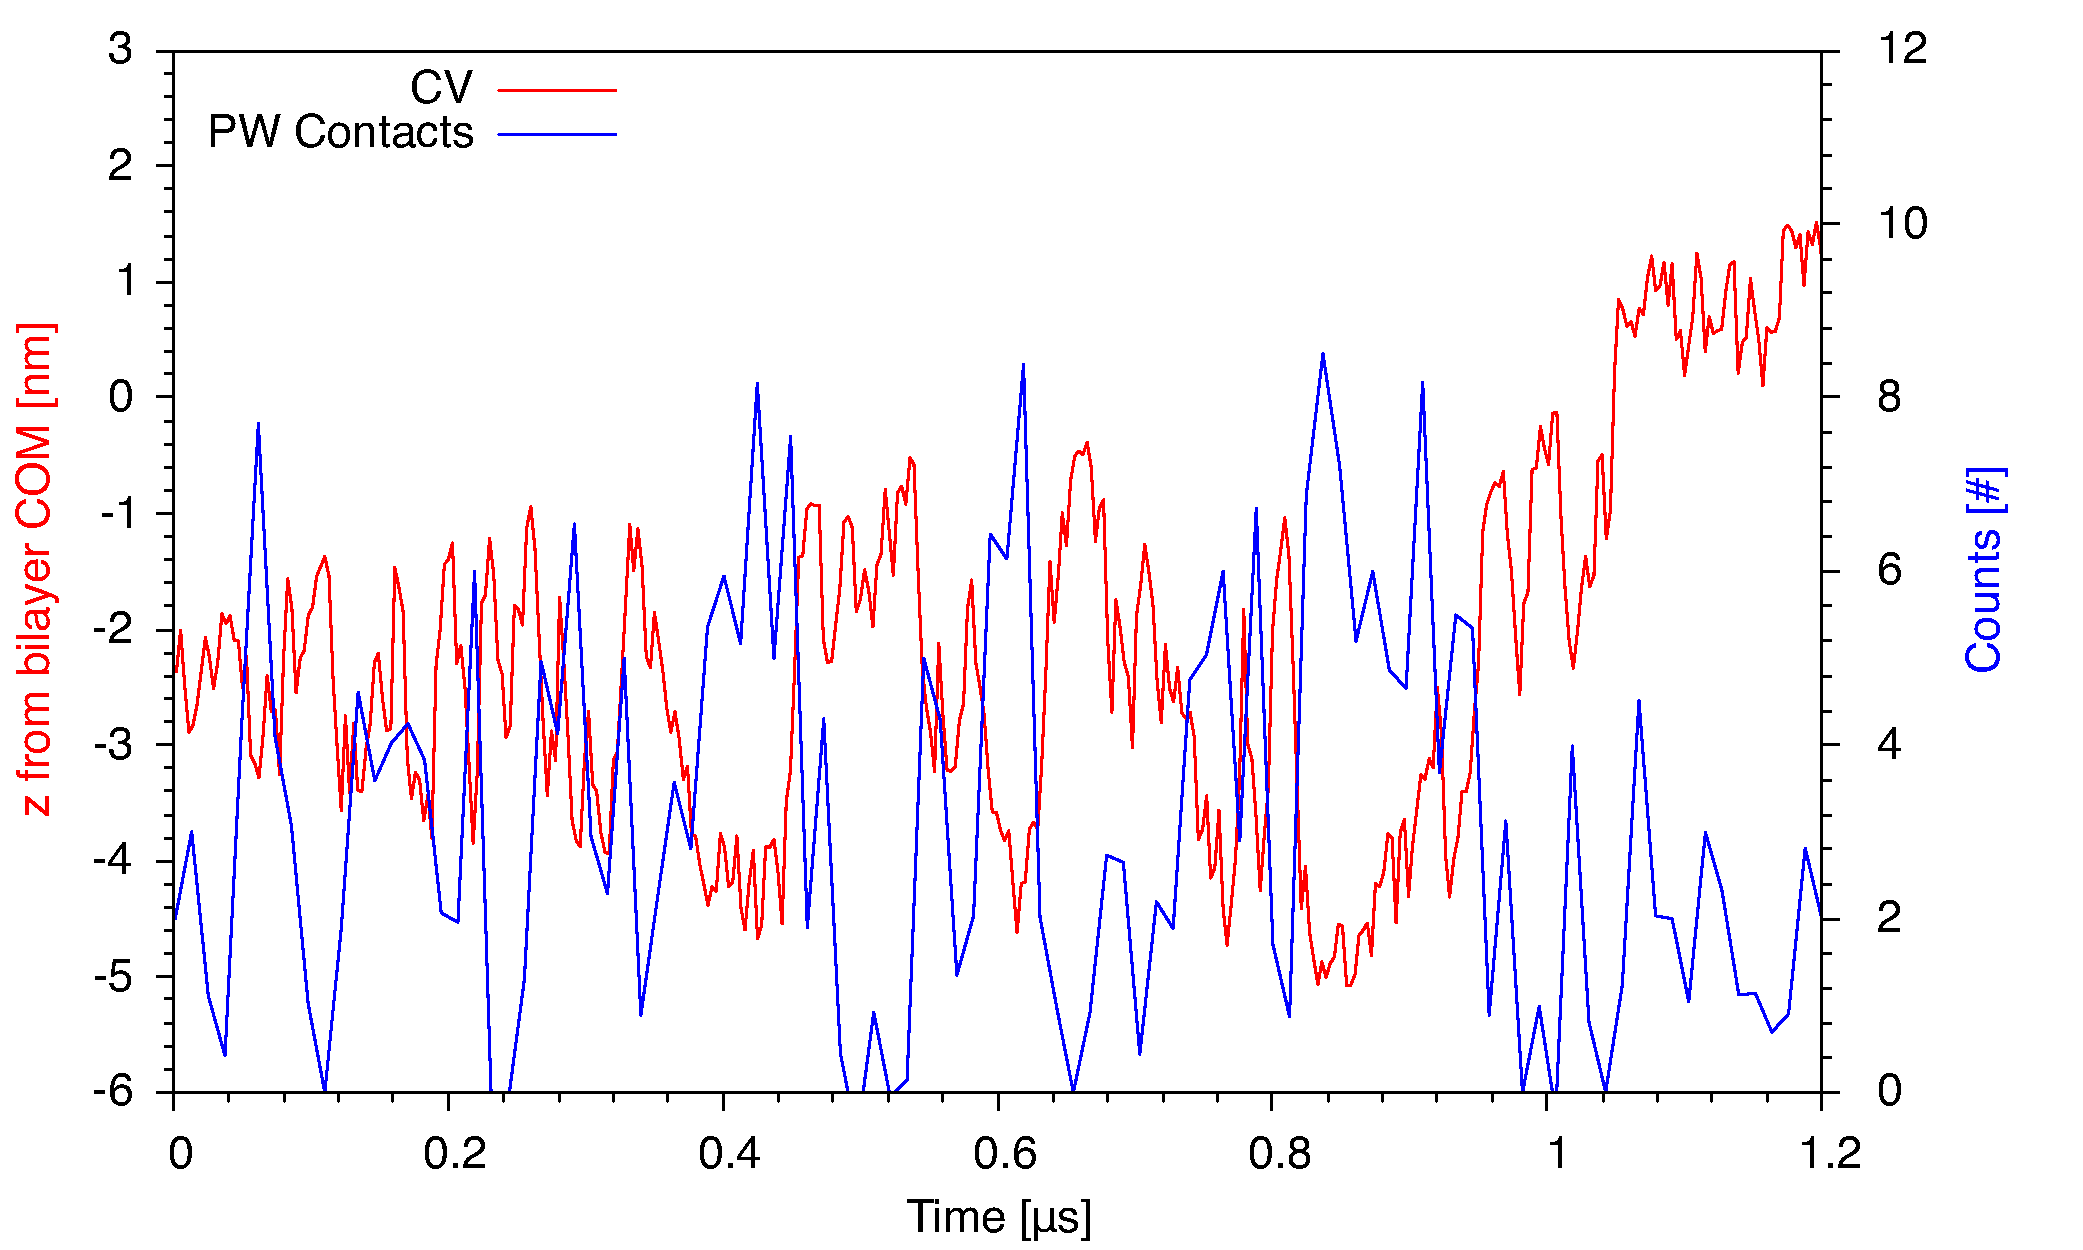
\includegraphics[width=0.9\textwidth]{./img/results/wCorrelation}
	\caption{Superposition of the \acs{CV} (red) and the number of contacts between the \acs{PW} beads and the charged bead (blue) in function of the time for a striped metadyamcis run. $z>0$ corresponds to the anchored state. It can be noted a clear anti--correlation between the distance of the charged bead from the bilayer \acs{COM} and the number of the \acs{PW} contacts: they decrease when the charged bead is approaching the hydrophobic region.}
\end{figure}

%	WPatchedComparison		WRPComparison
\newgeometry{left=2.5cm,right=2.5cm}
\begin{figure}
	\center
	\subfloat[striped – model comparison]{
		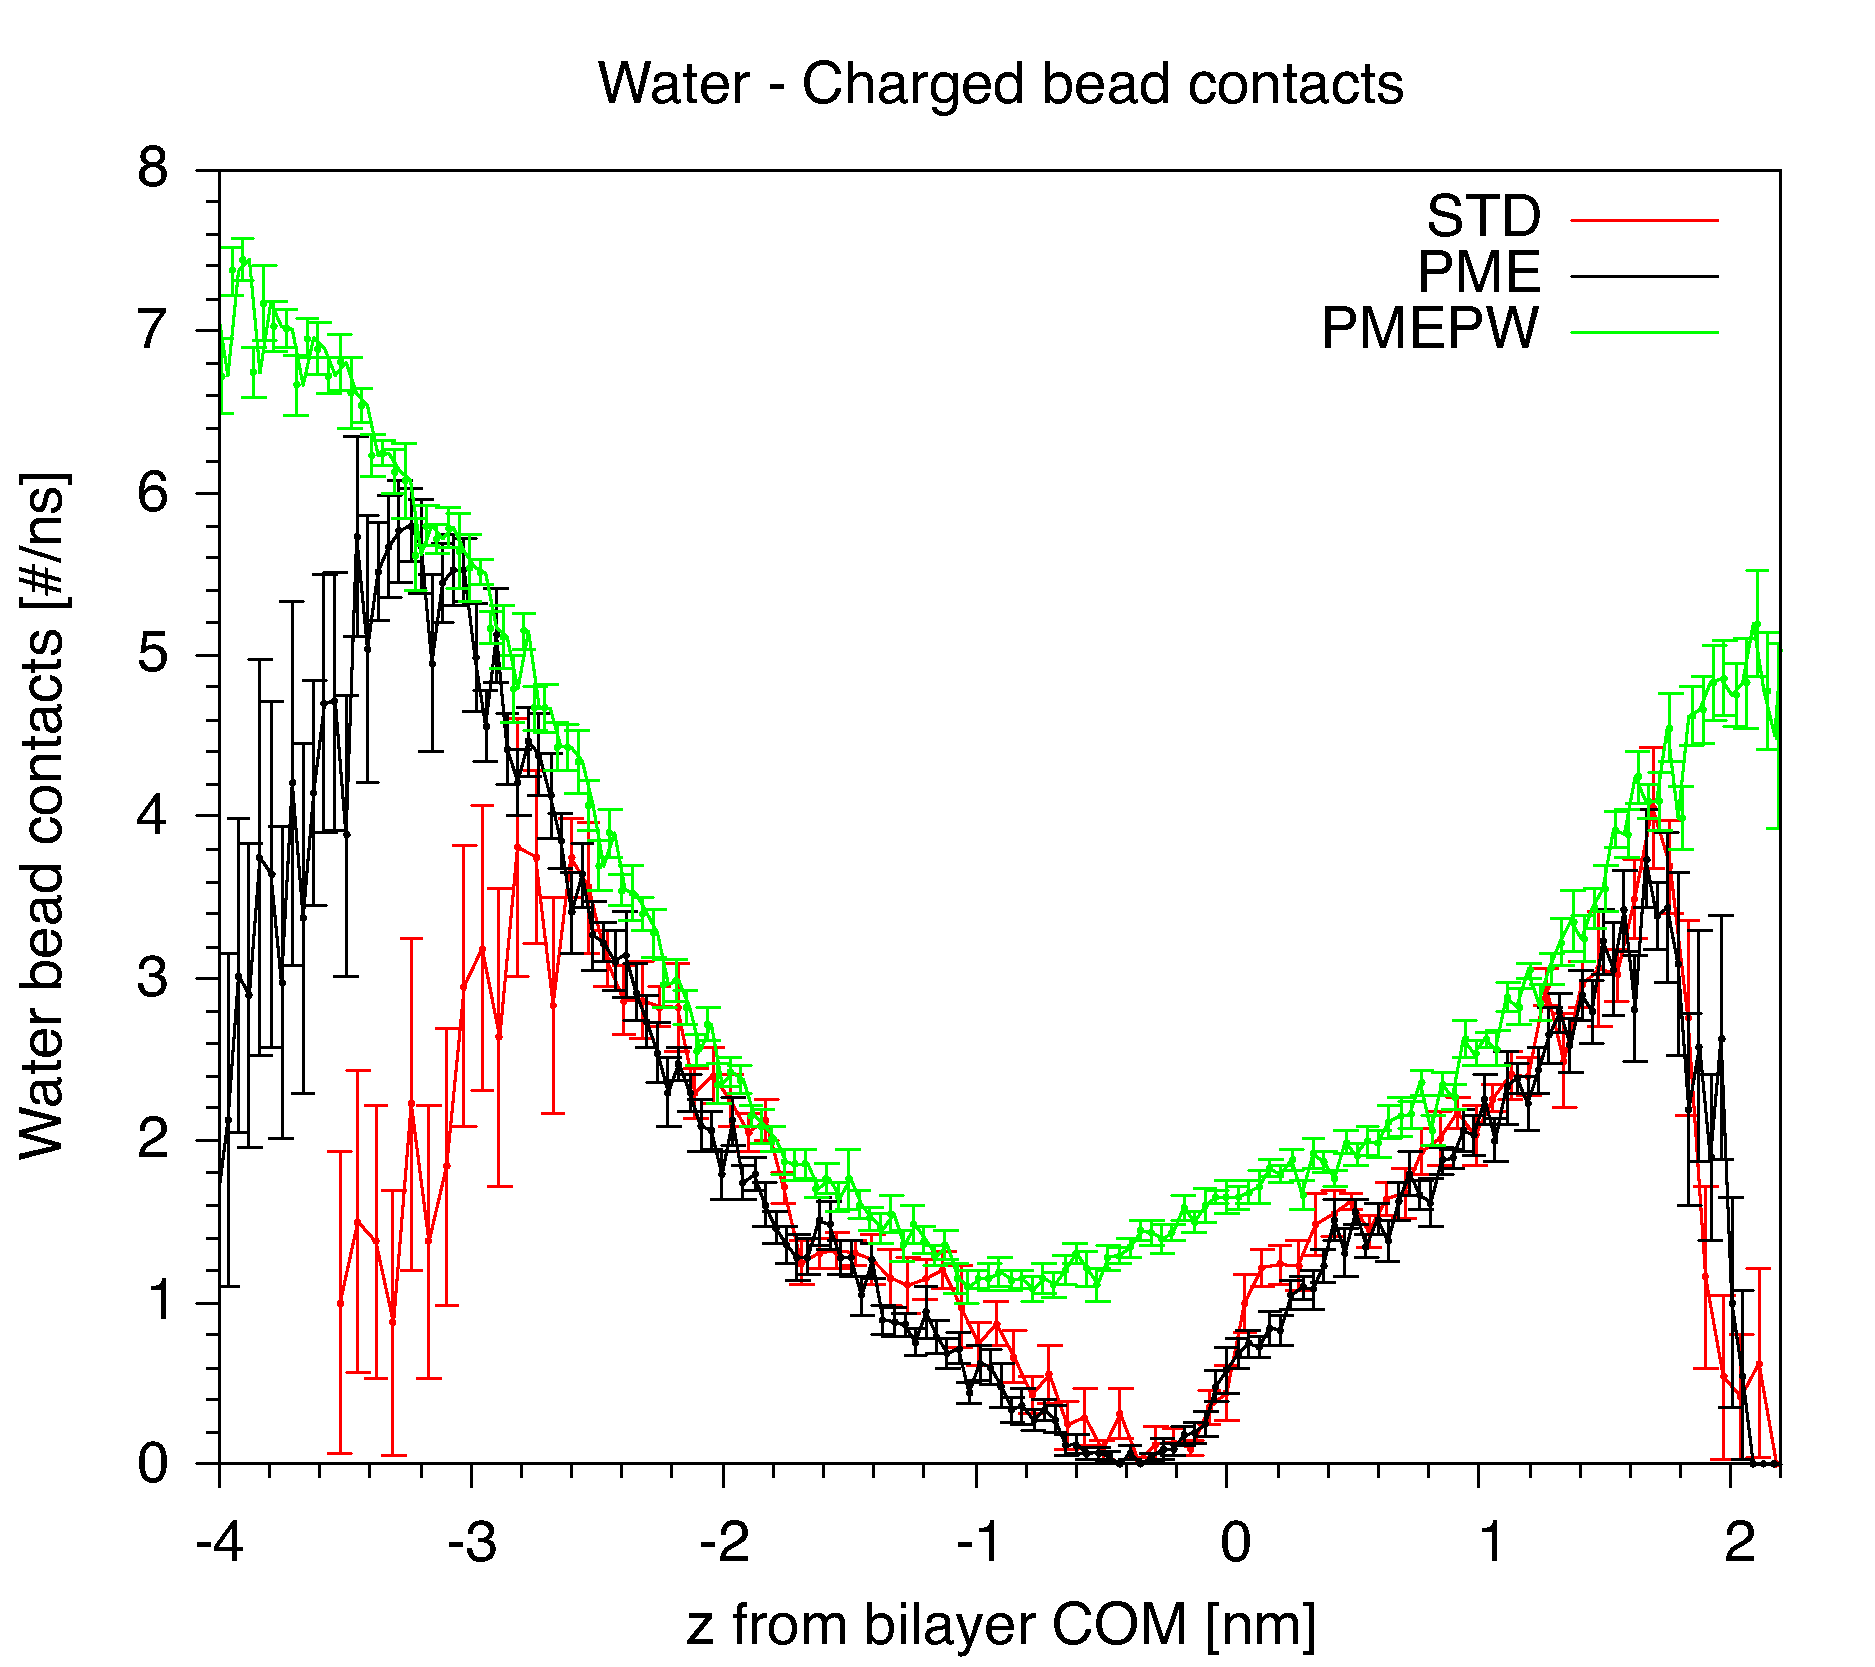
\includegraphics[width=0.5\textwidth]{./img/results/WPatchedComparison}
	}%
	\subfloat[striped – random comparison]{
		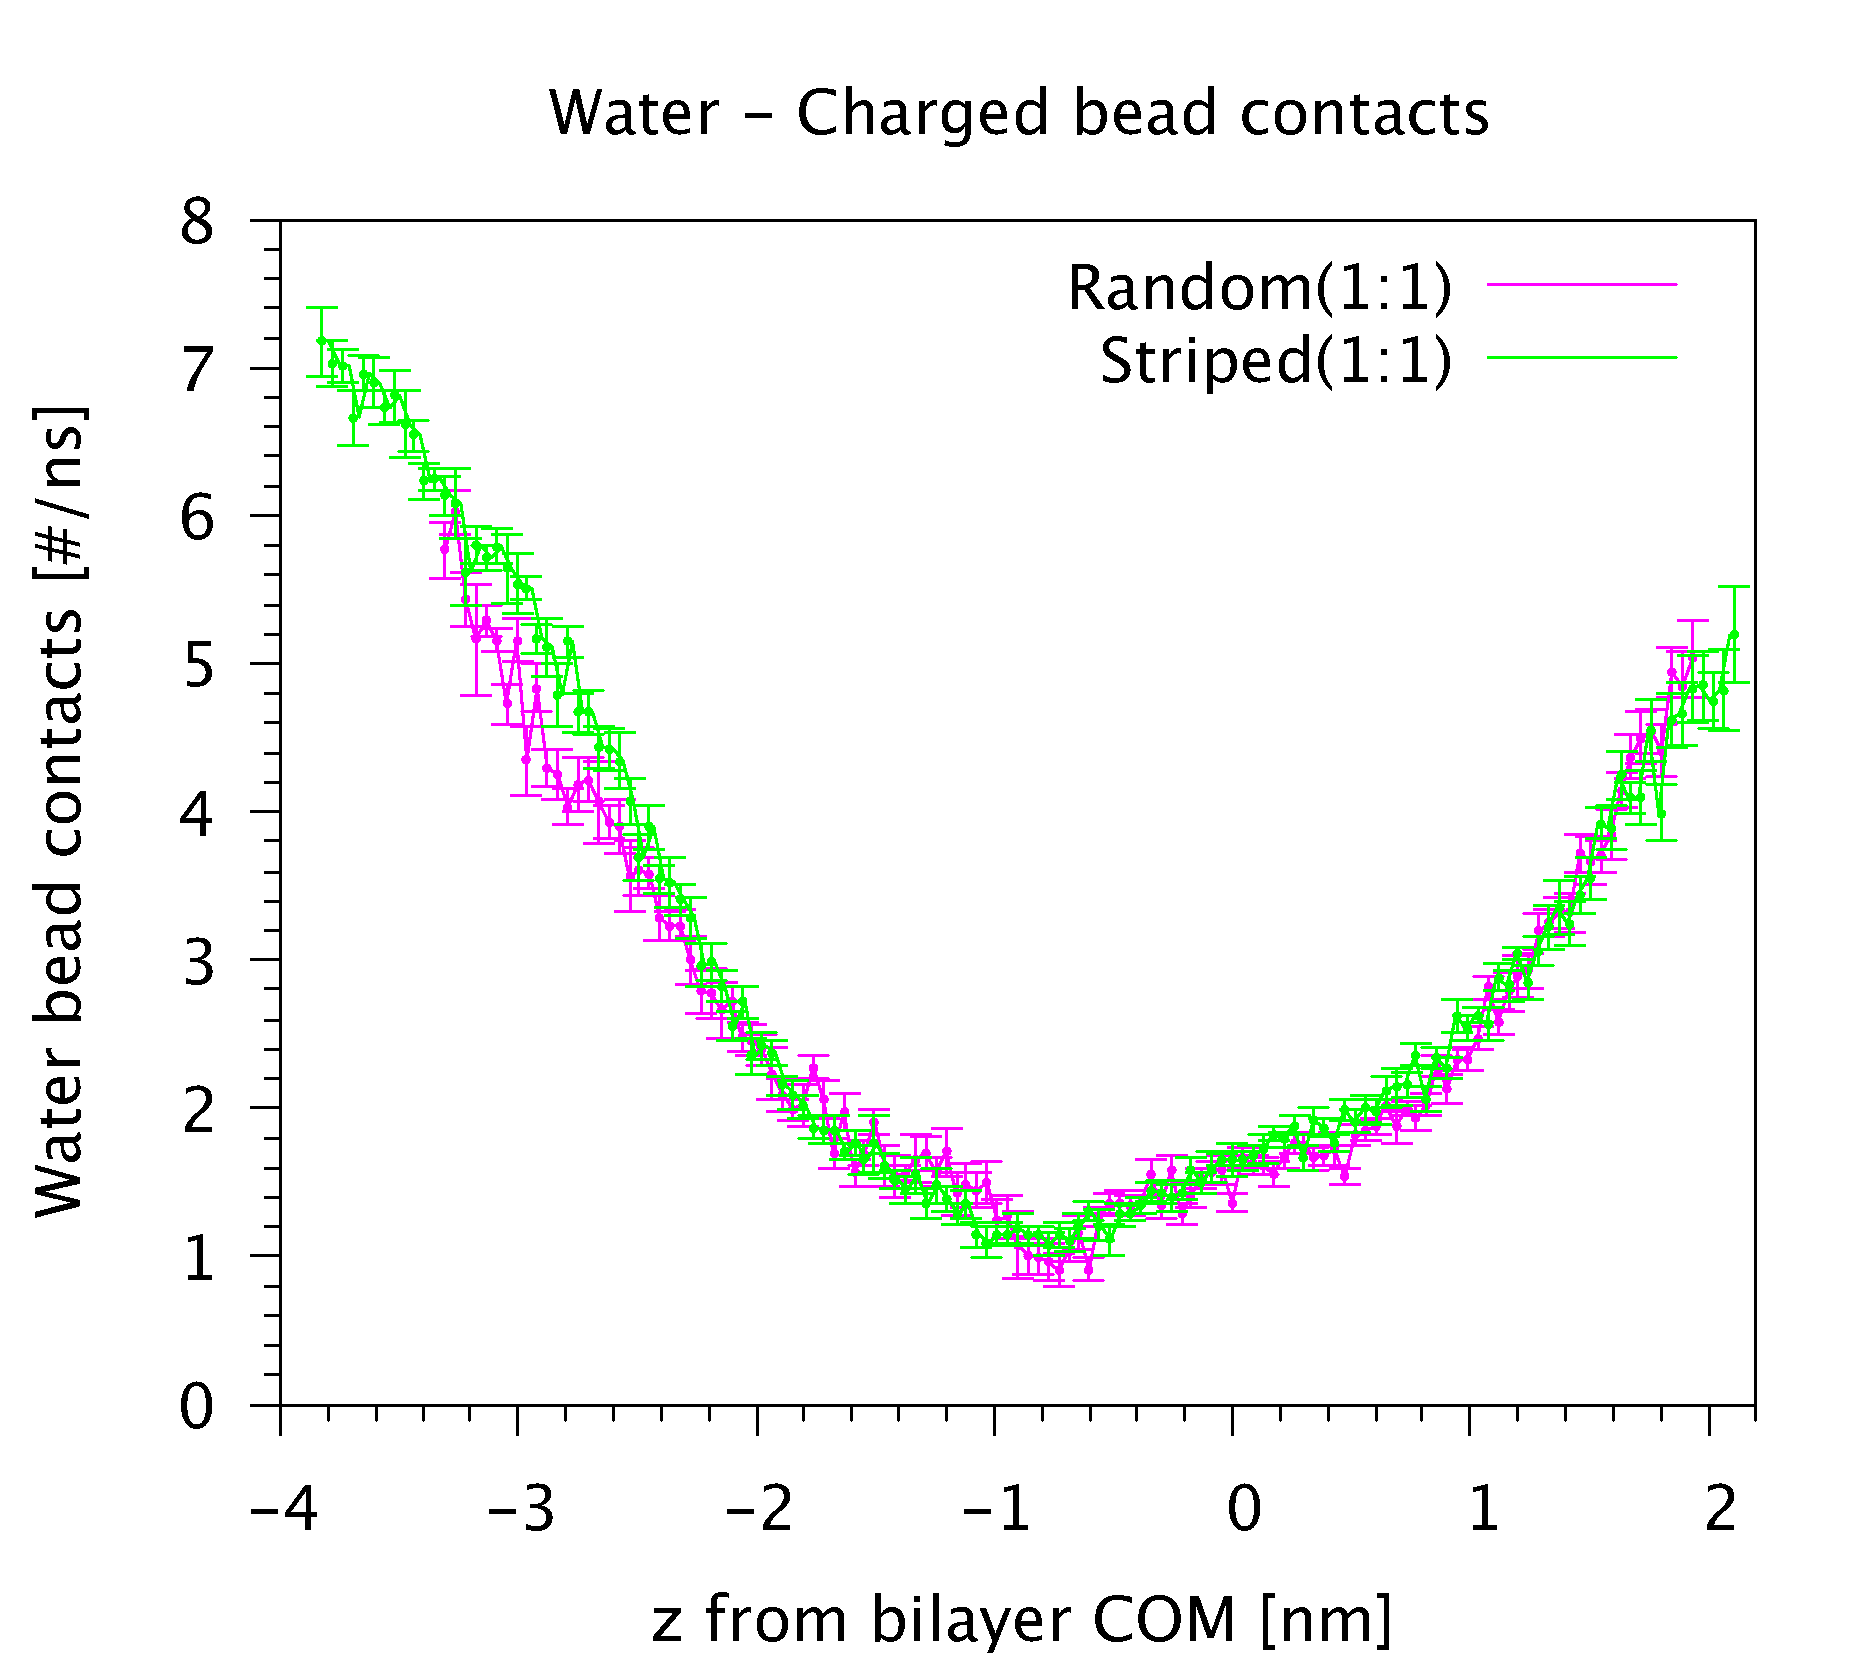
\includegraphics[width=0.5\textwidth]{./img/results/WRPComparison}
	}%
	\caption{Number of contacts per ns between water beads and the charged bead in function of the position of the charged bead. (a) For the striped \acs{NP} in comparison with different models. (b) In comparison between the striped and the random \acs{NP}s.}
\end{figure}
\restoregeometry

\section{Lipid heads dragging}
%Trascinamento delle teste dei lipidi nelle varie salse

% 	minDistPatched			minDistRandom11
\begin{figure}[p]
	\center
	\subfloat[striped NP]{
		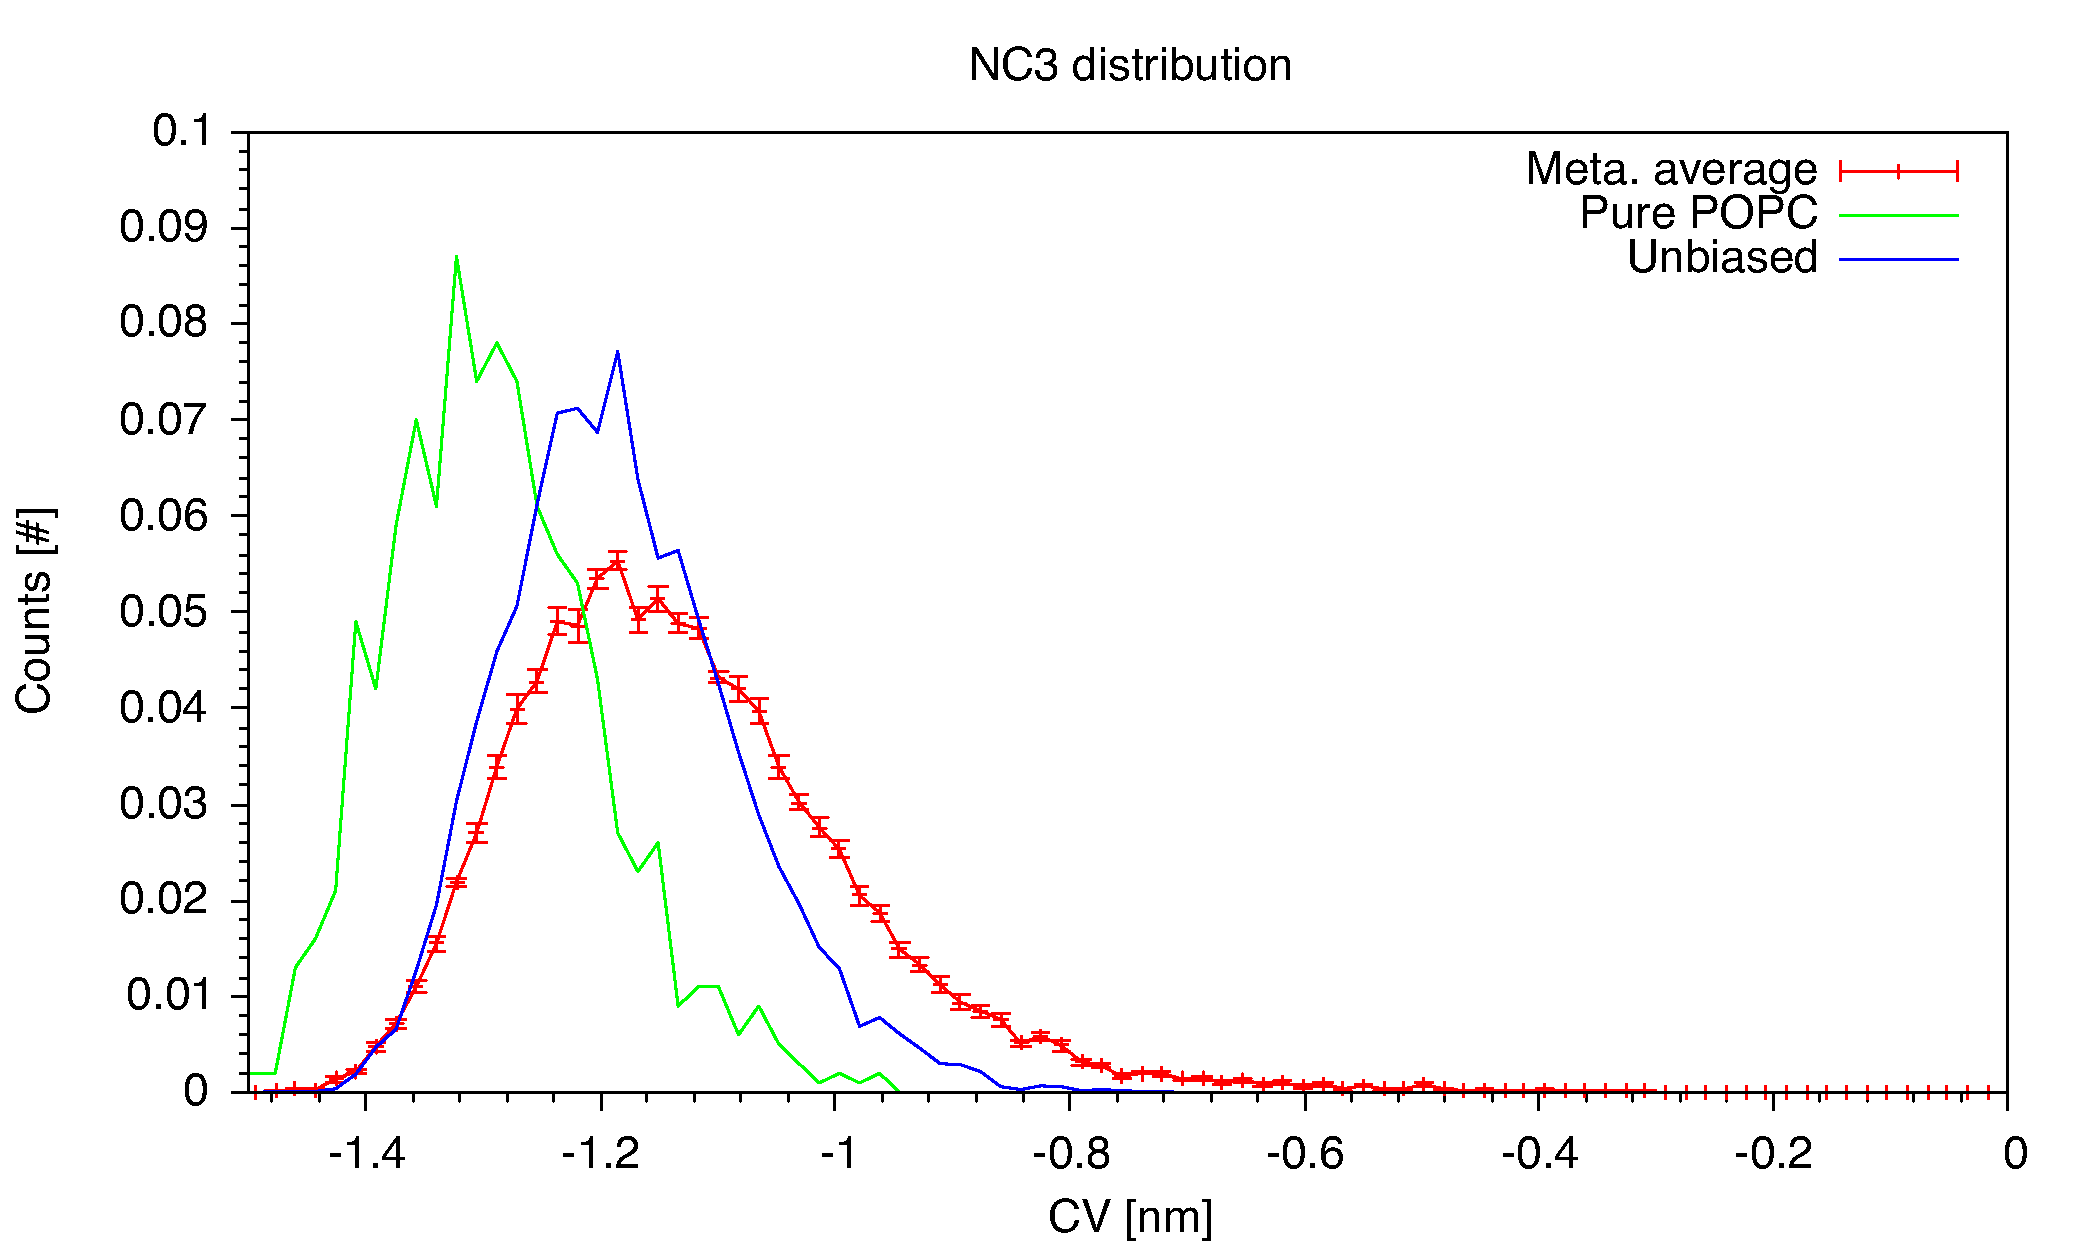
\includegraphics[width=\textwidth]{./img/results/minDistPatched}
	}\\%
	\subfloat[random NP]{
		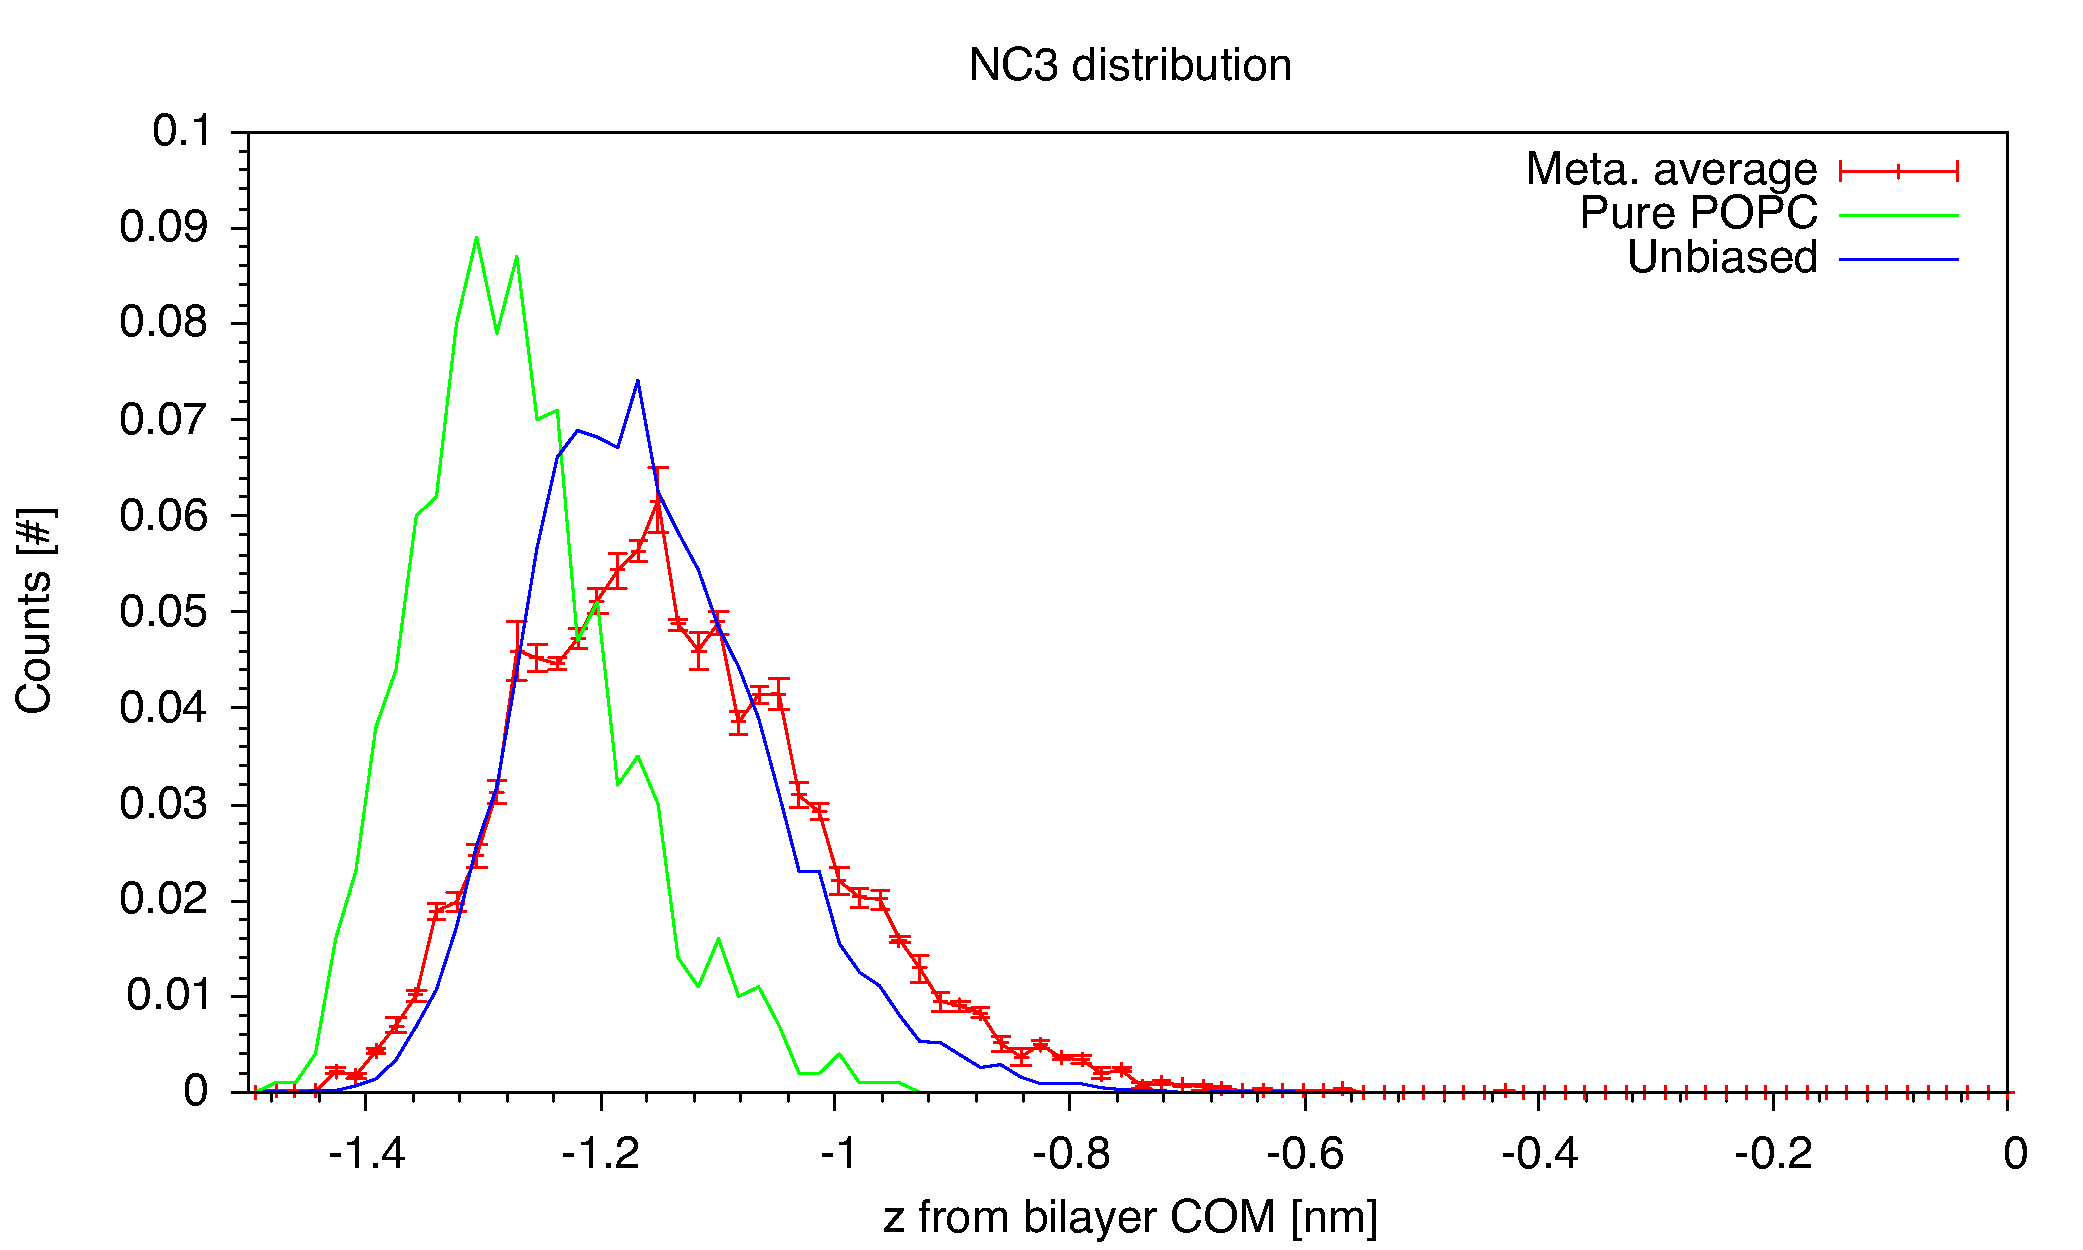
\includegraphics[width=\textwidth]{./img/results/minDistRandom11}
	}%
	\caption{Average distribution of the coline groups (NC3 beads) in the entrance leaflet closer to the bilayer \acs{COM} in function of the position of the charged bead in comparison with an average over ten metadynamics runs, the unbiased run and a pure \acs{POPC} run for: (a) the striped \acs{NP}; (b) the random \acs{NP}.}
\end{figure}

%	NC3PatchedComparison	NC3RPComparison
\newgeometry{left=2.5cm,right=2.5cm}
\begin{figure}
	\center
	\subfloat[striped – model comparison]{
		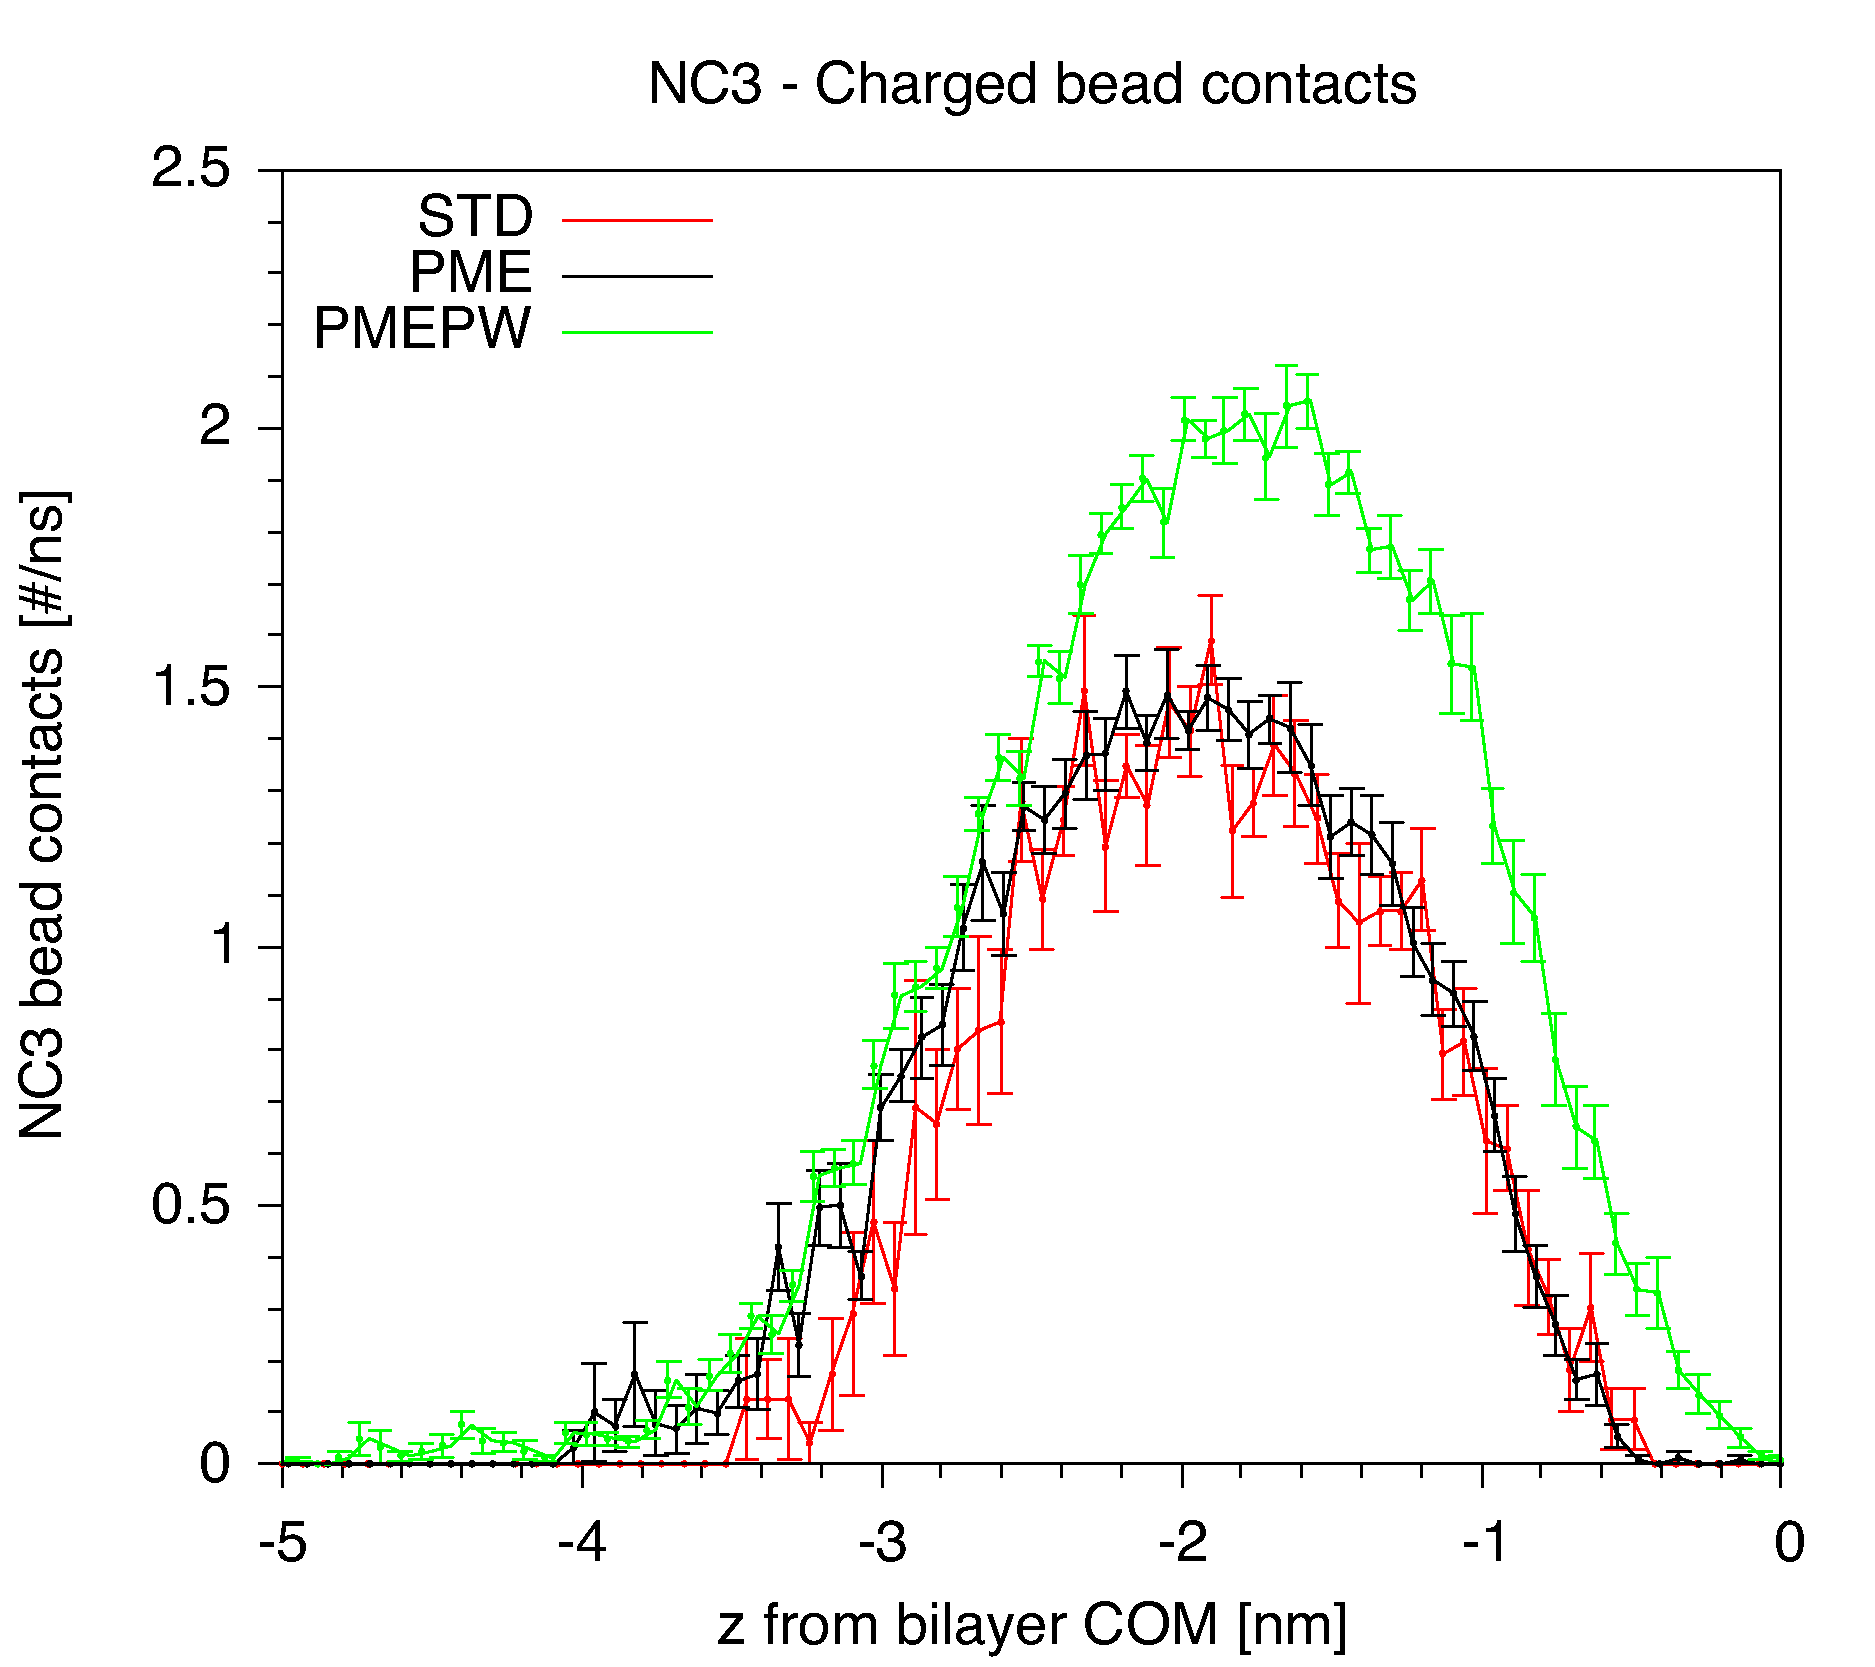
\includegraphics[width=0.5\textwidth]{./img/results/NC3PatchedComparison}
	}%
	\subfloat[striped – random comparison]{
		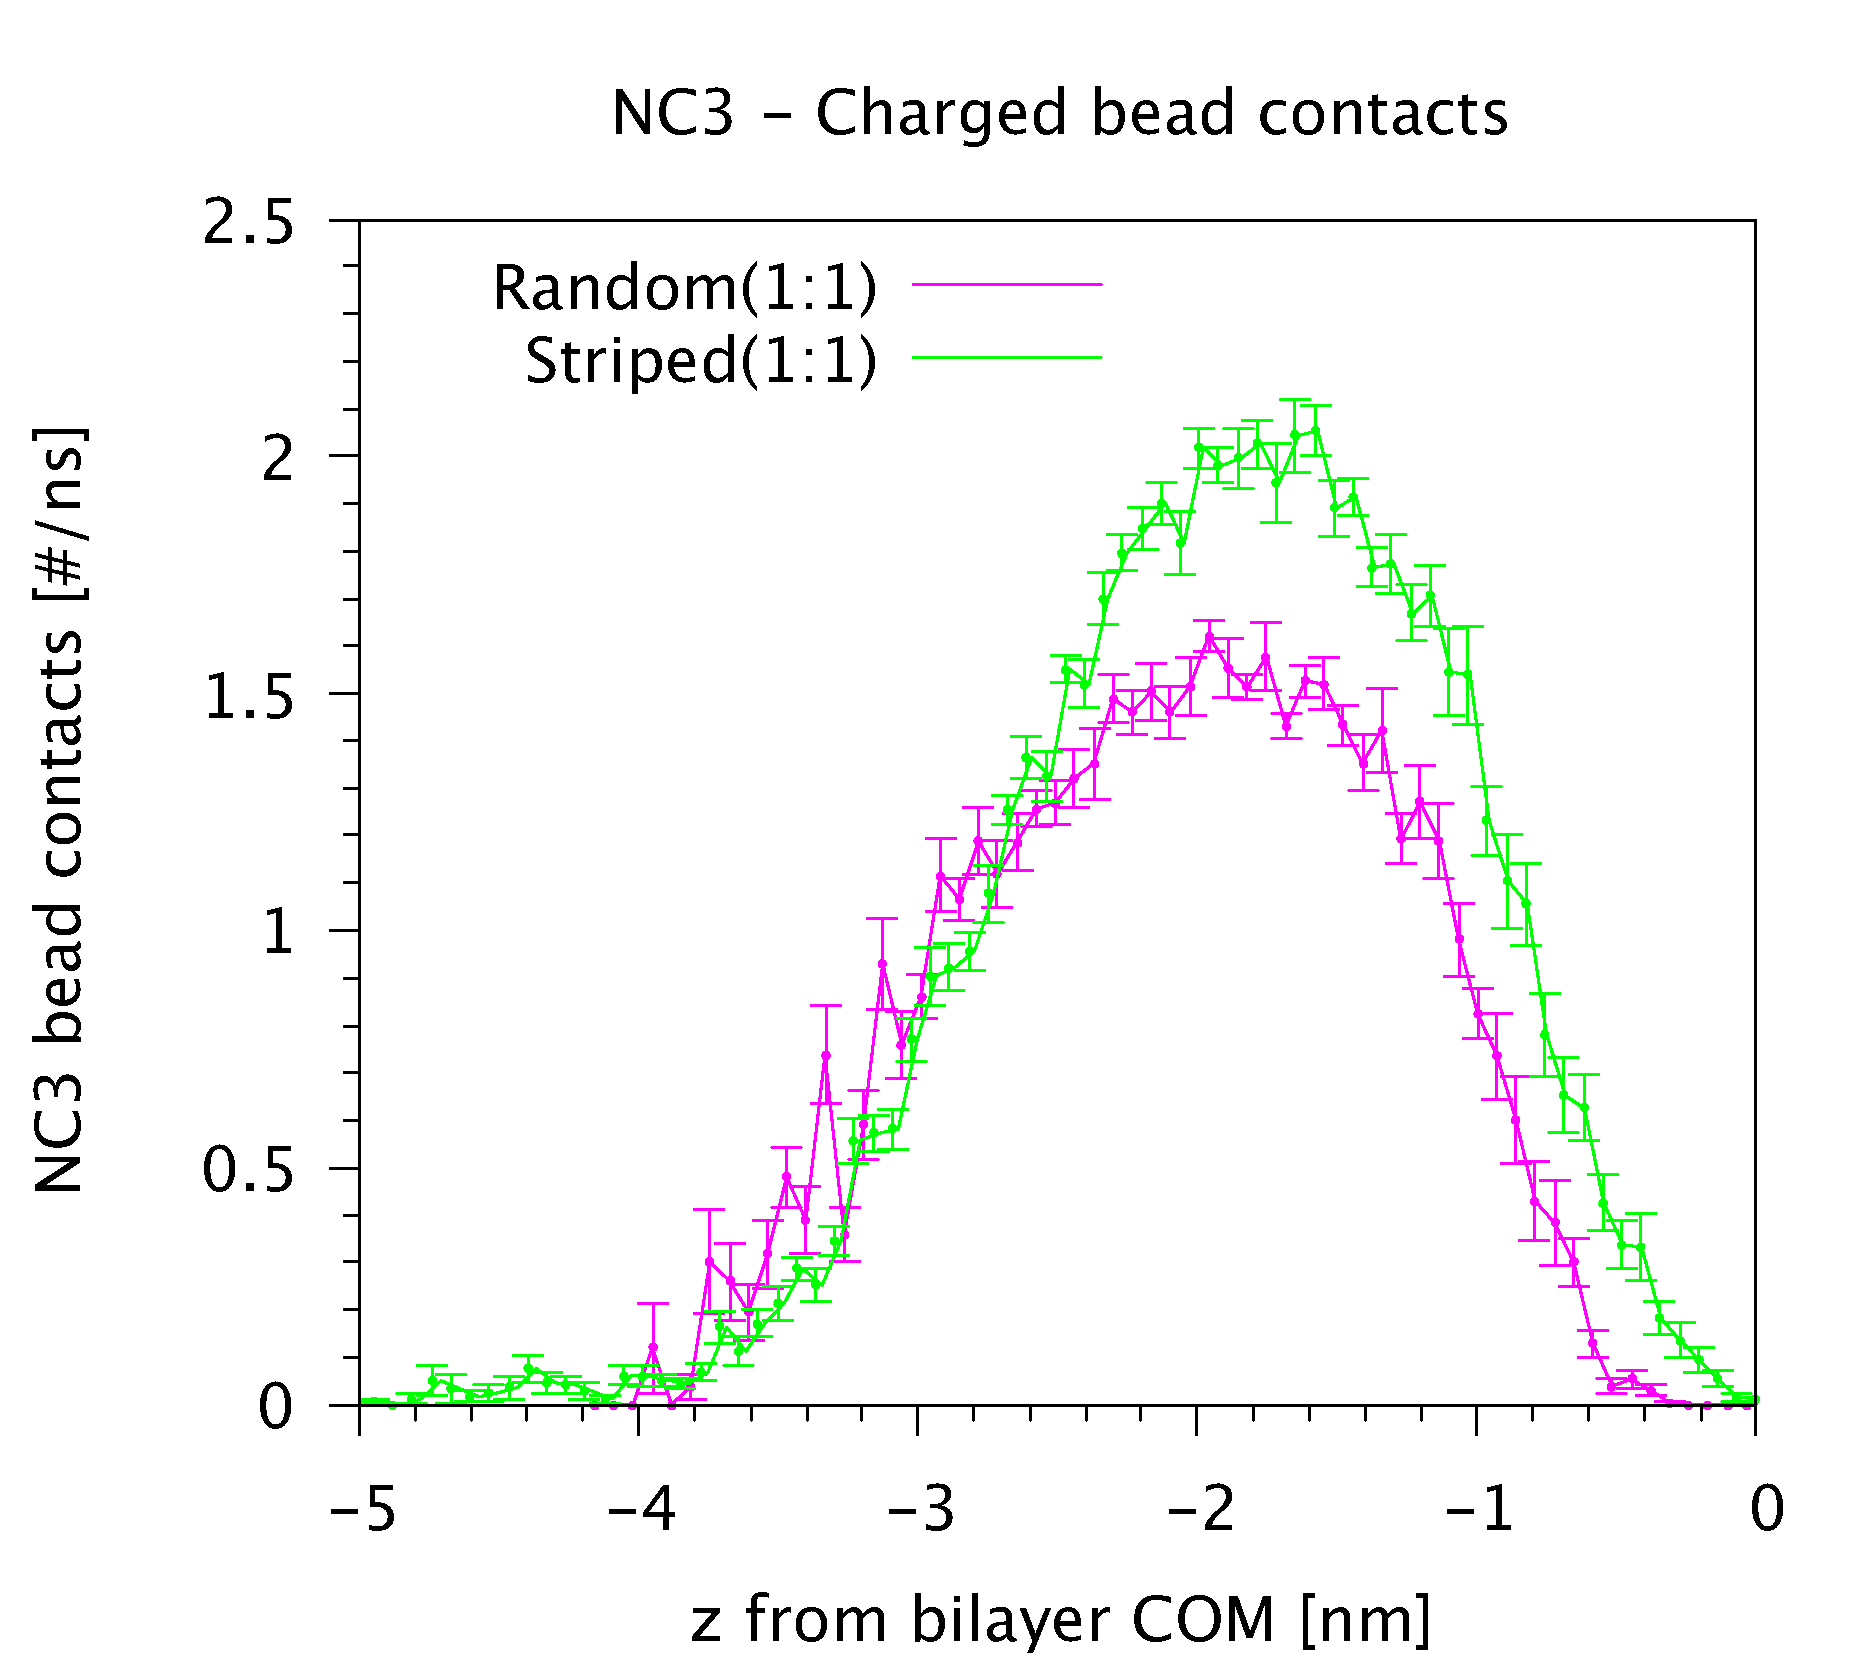
\includegraphics[width=0.5\textwidth]{./img/results/NC3RPComparison}
	}%
	\caption{Number of contacts per ns between coline group (NC3 bead) and the charged bead in function of the position of the charged bead in the hydrophobic state. (a) For the striped \acs{NP} in comparison with different models. (b) In comparison between the striped and the random \acs{NP}s.}
\end{figure}
\restoregeometry

\section{Effects of metadynamics}
%Quanto la metadinamica sia distrittiva: comparazione tra rum unbiased e biased

% 	minDistHydroPatched		minDistHydroRandom11
\begin{figure}[p]
	\center
	\subfloat[striped NP]{
		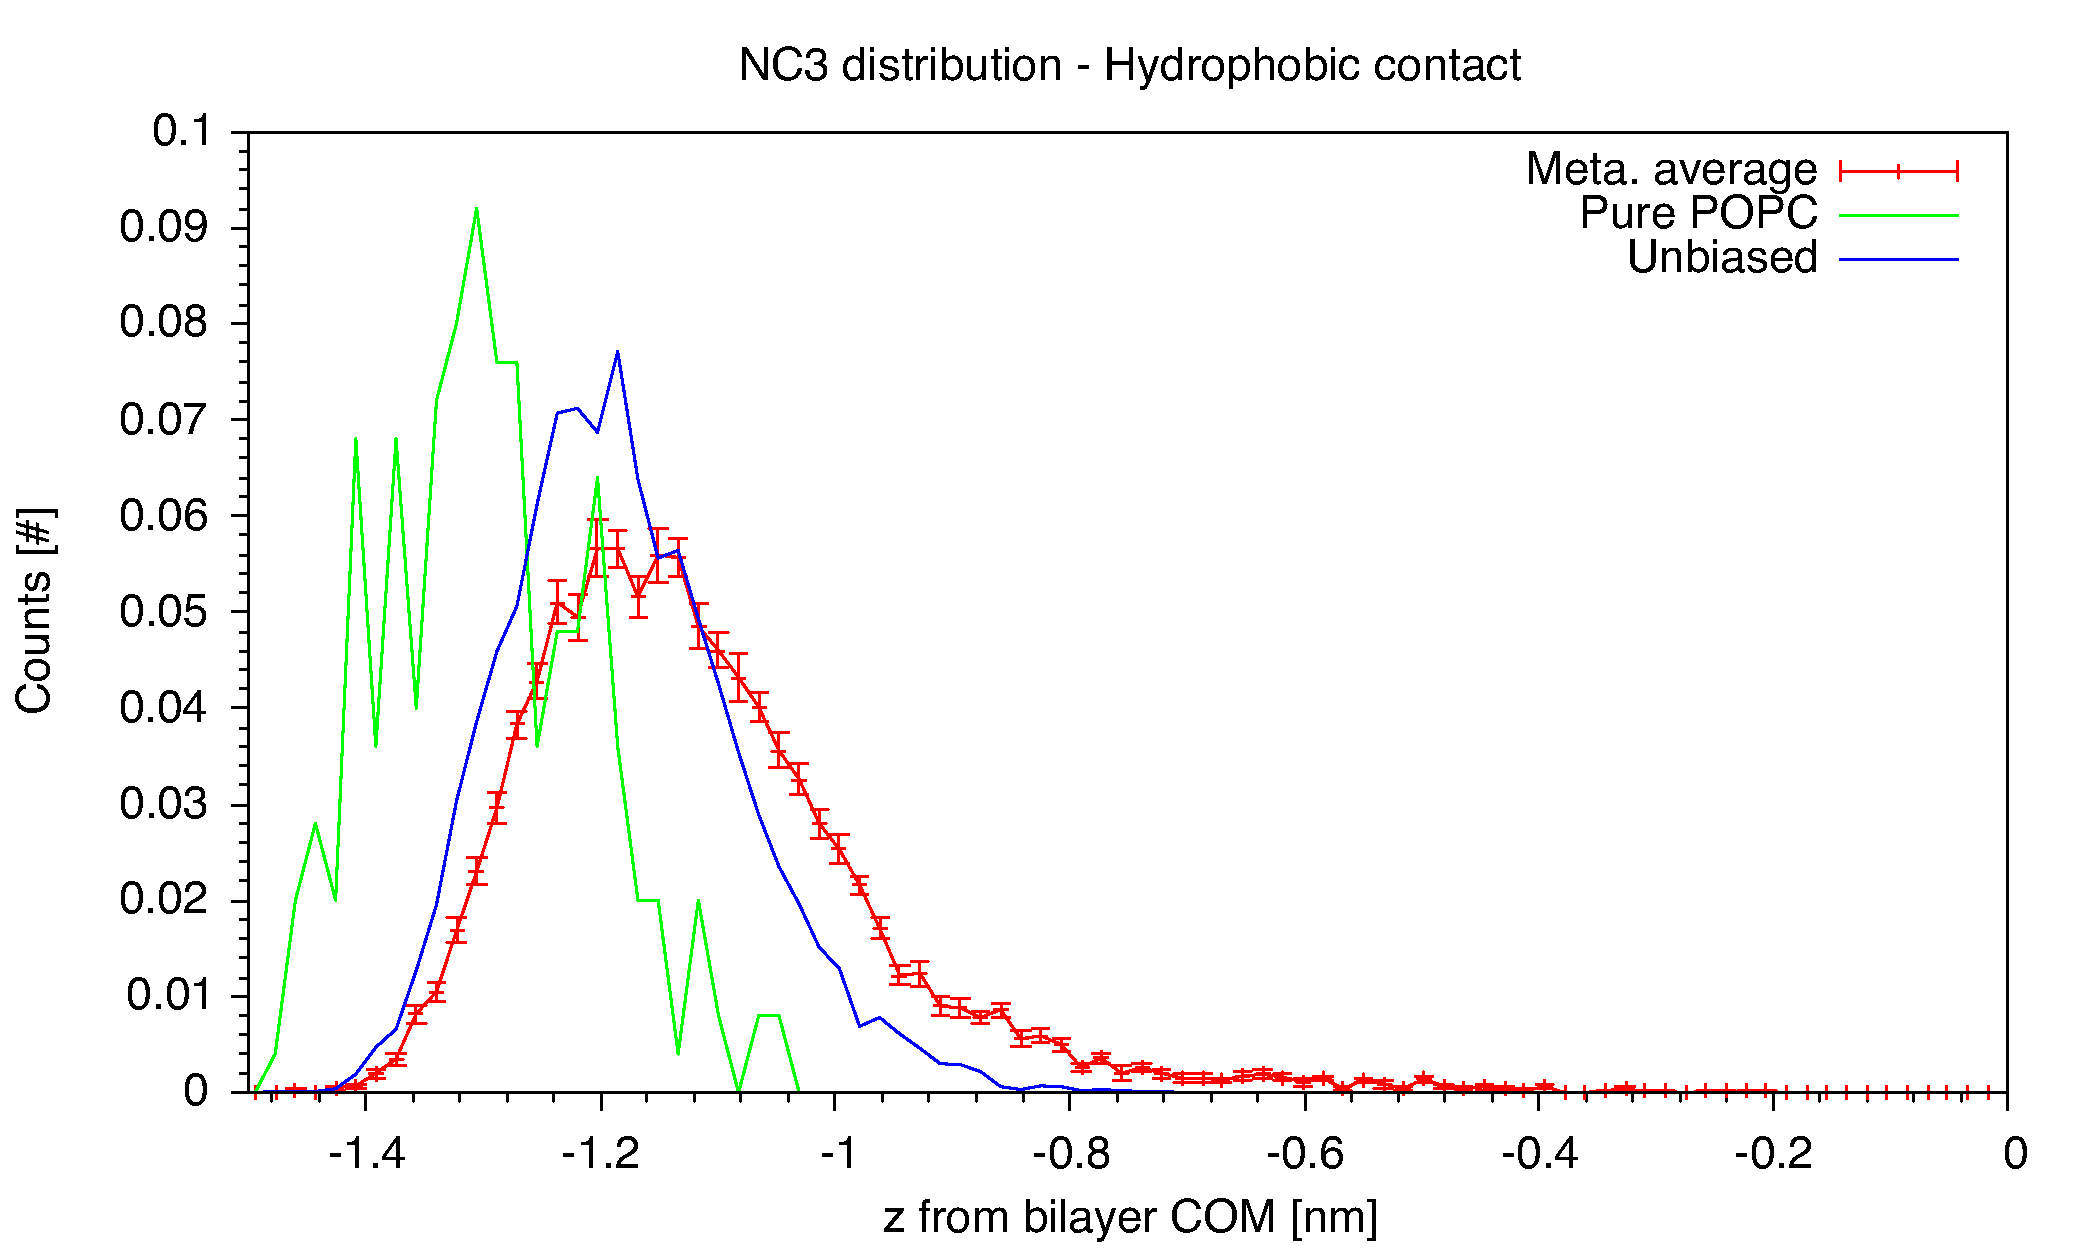
\includegraphics[width=\textwidth]{./img/results/minDistHydroPatched}
	}\\%
	\subfloat[random NP]{
		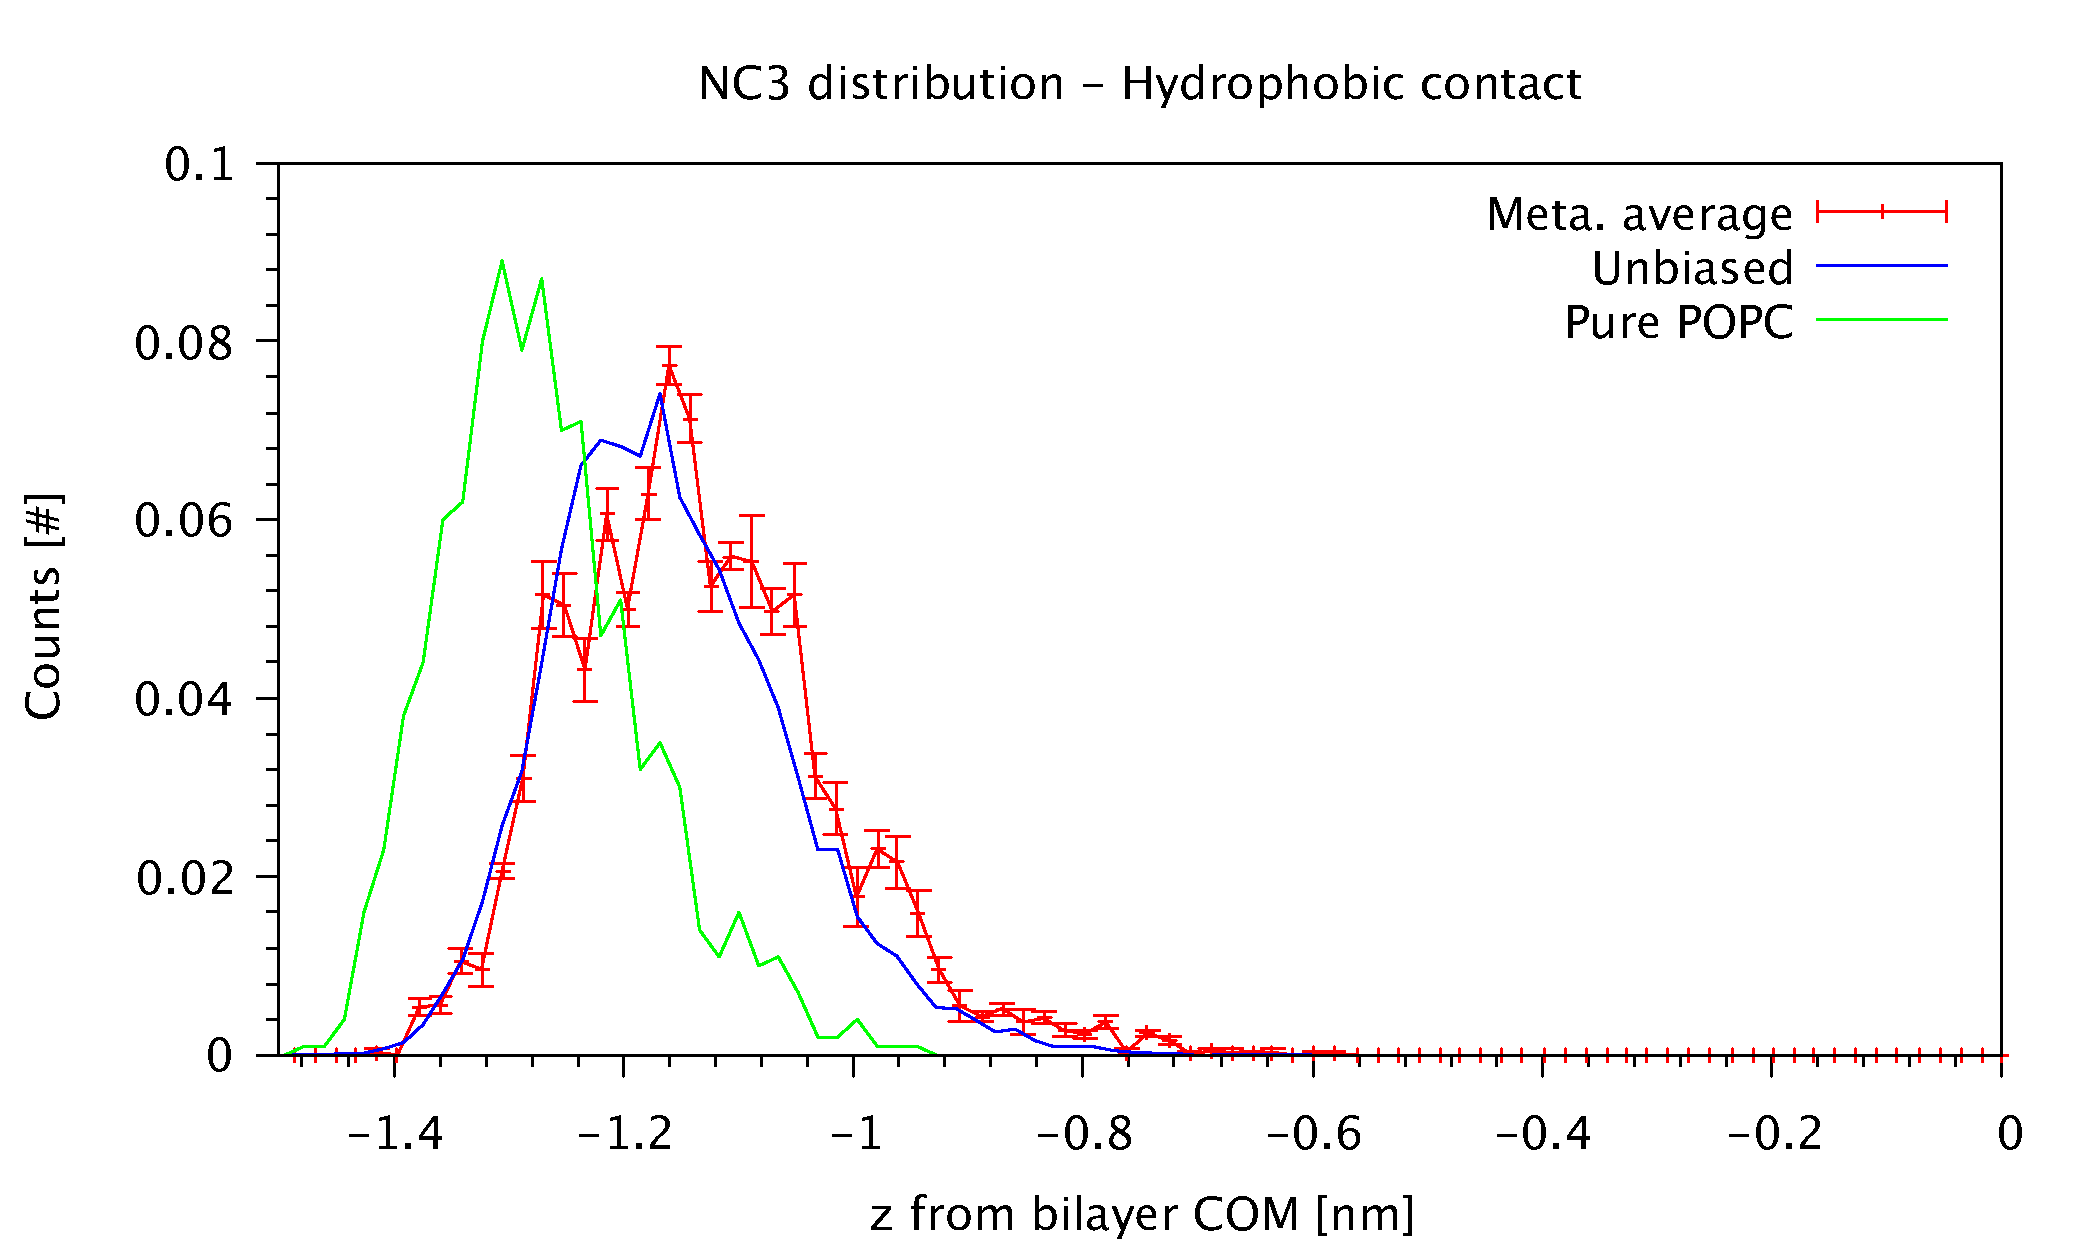
\includegraphics[width=\textwidth]{./img/results/minDistHydroRandom11}
	}%
	\caption{Average distribution of the coline groups (NC3 beads) in the entrance leaflet closer to the bilayer \acs{COM} in function of the position of the charged bead in the hydrophobic state and in comparison with an average over ten metadynamics runs in the hydrophobic contact only, the unbiased run and a pure \acs{POPC} run for: (a) the striped \acs{NP}; (b) the random \acs{NP}.}
\end{figure}

%	patchedPWContact	randon11PWContact
% 	patchedNC3Contact	random11NC3Contact
\newgeometry{left=2.5cm,right=2.5cm}
\begin{figure}[p]
	\center
	\subfloat[striped NP]{
		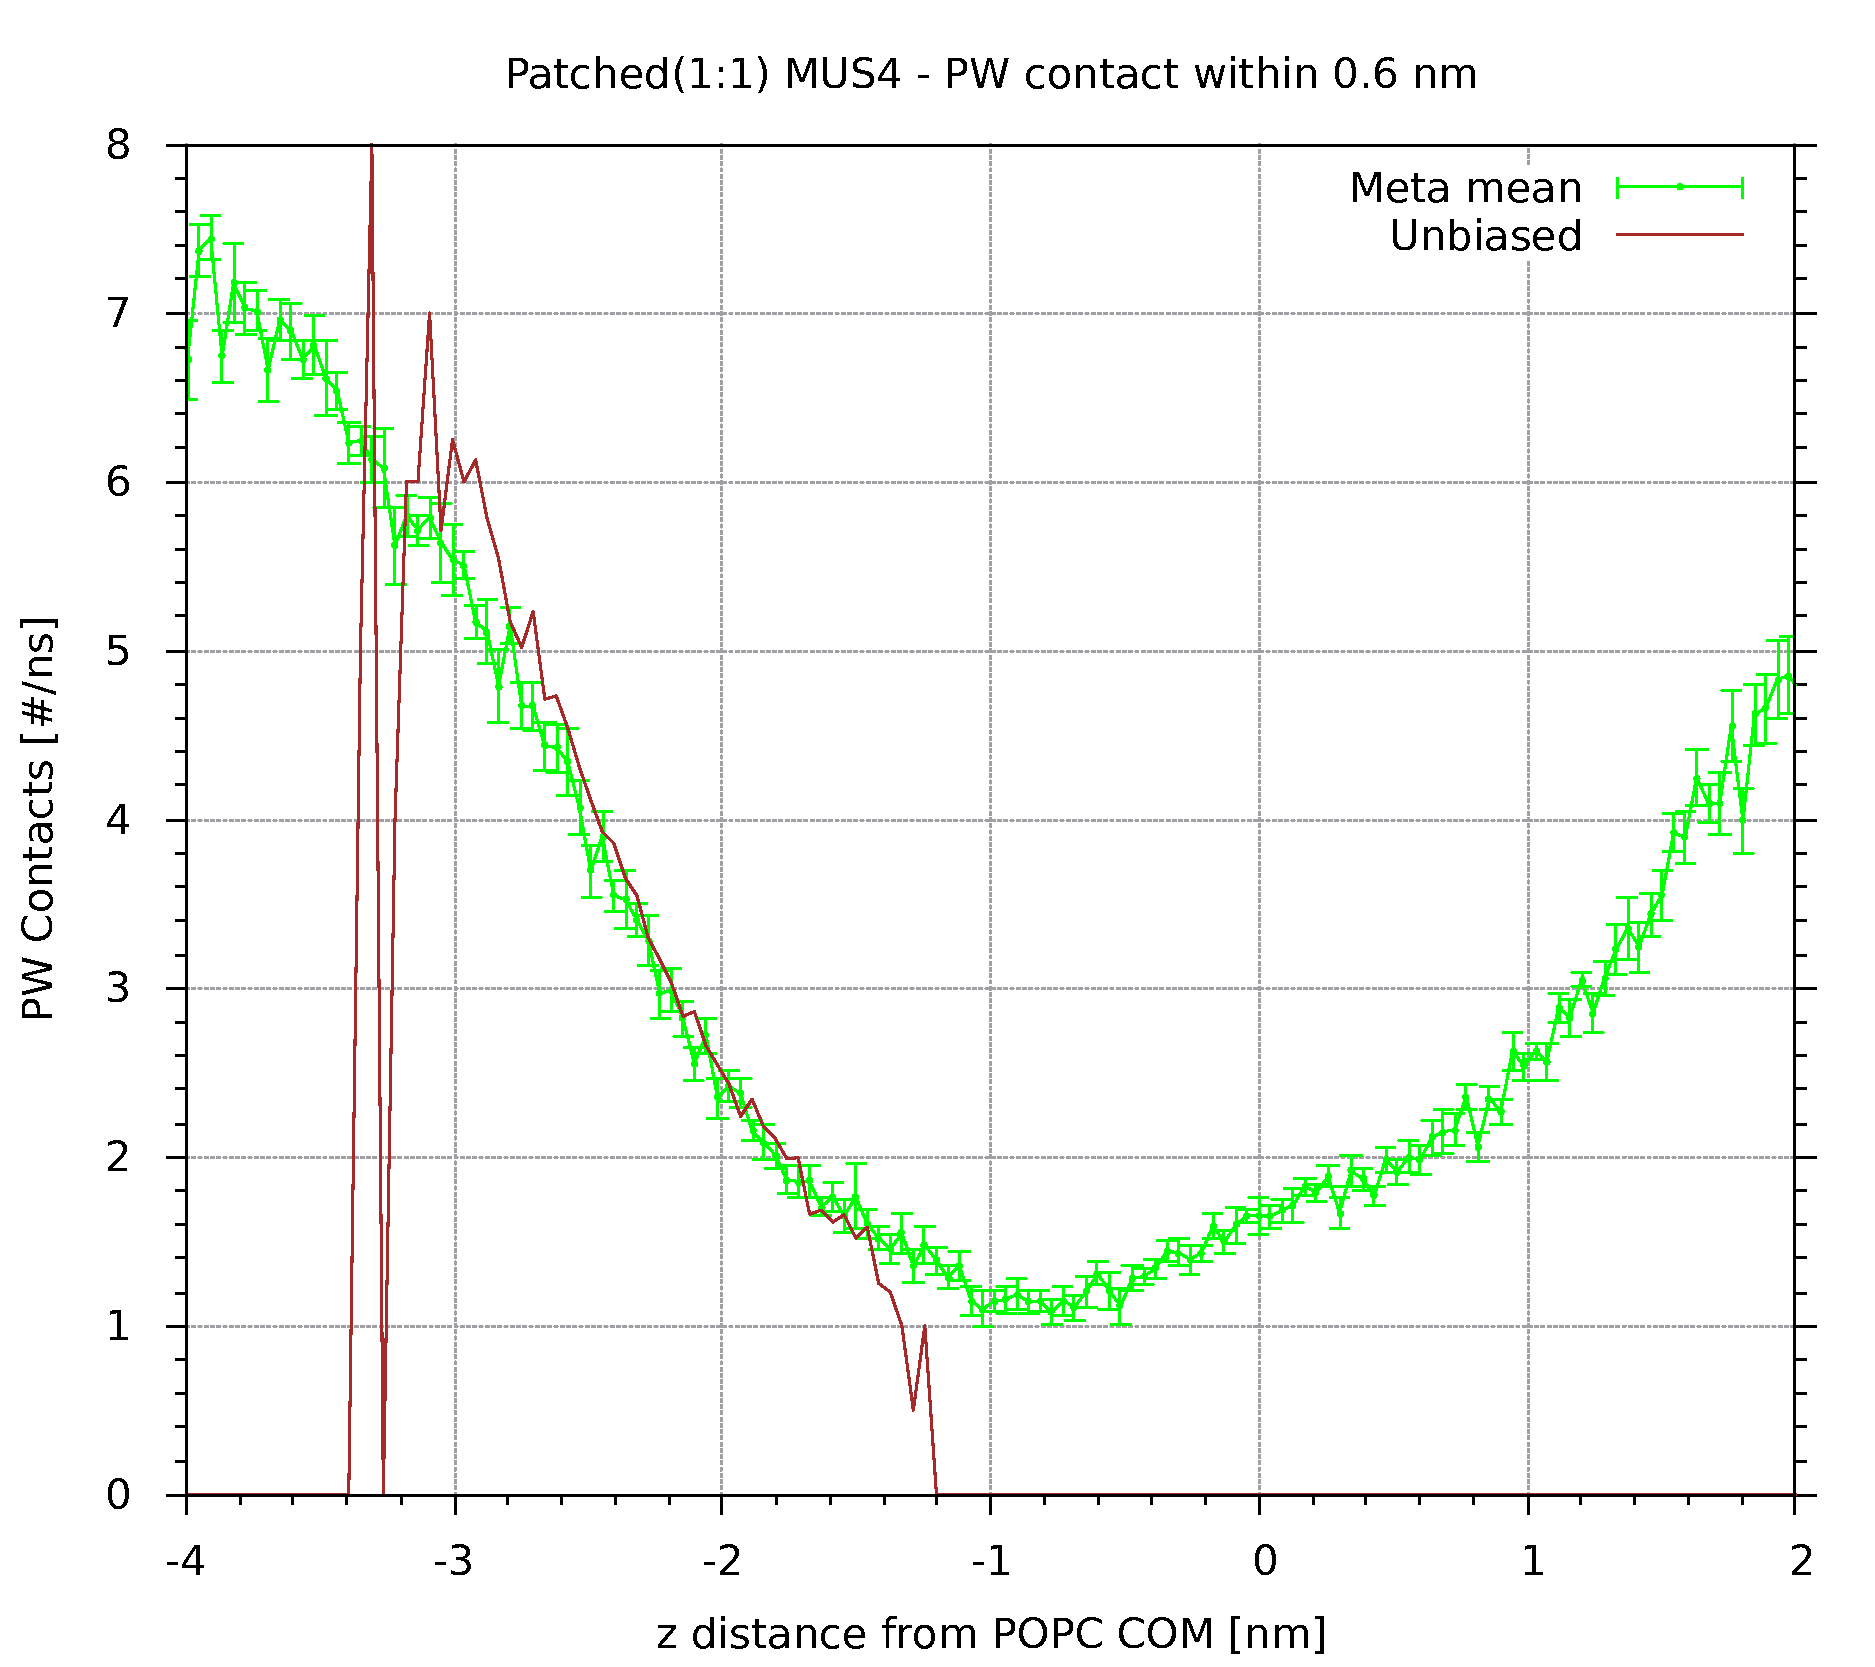
\includegraphics[width=0.5\textwidth]{./img/results/patchedPWContact}
	}%
	\subfloat[random NP]{
		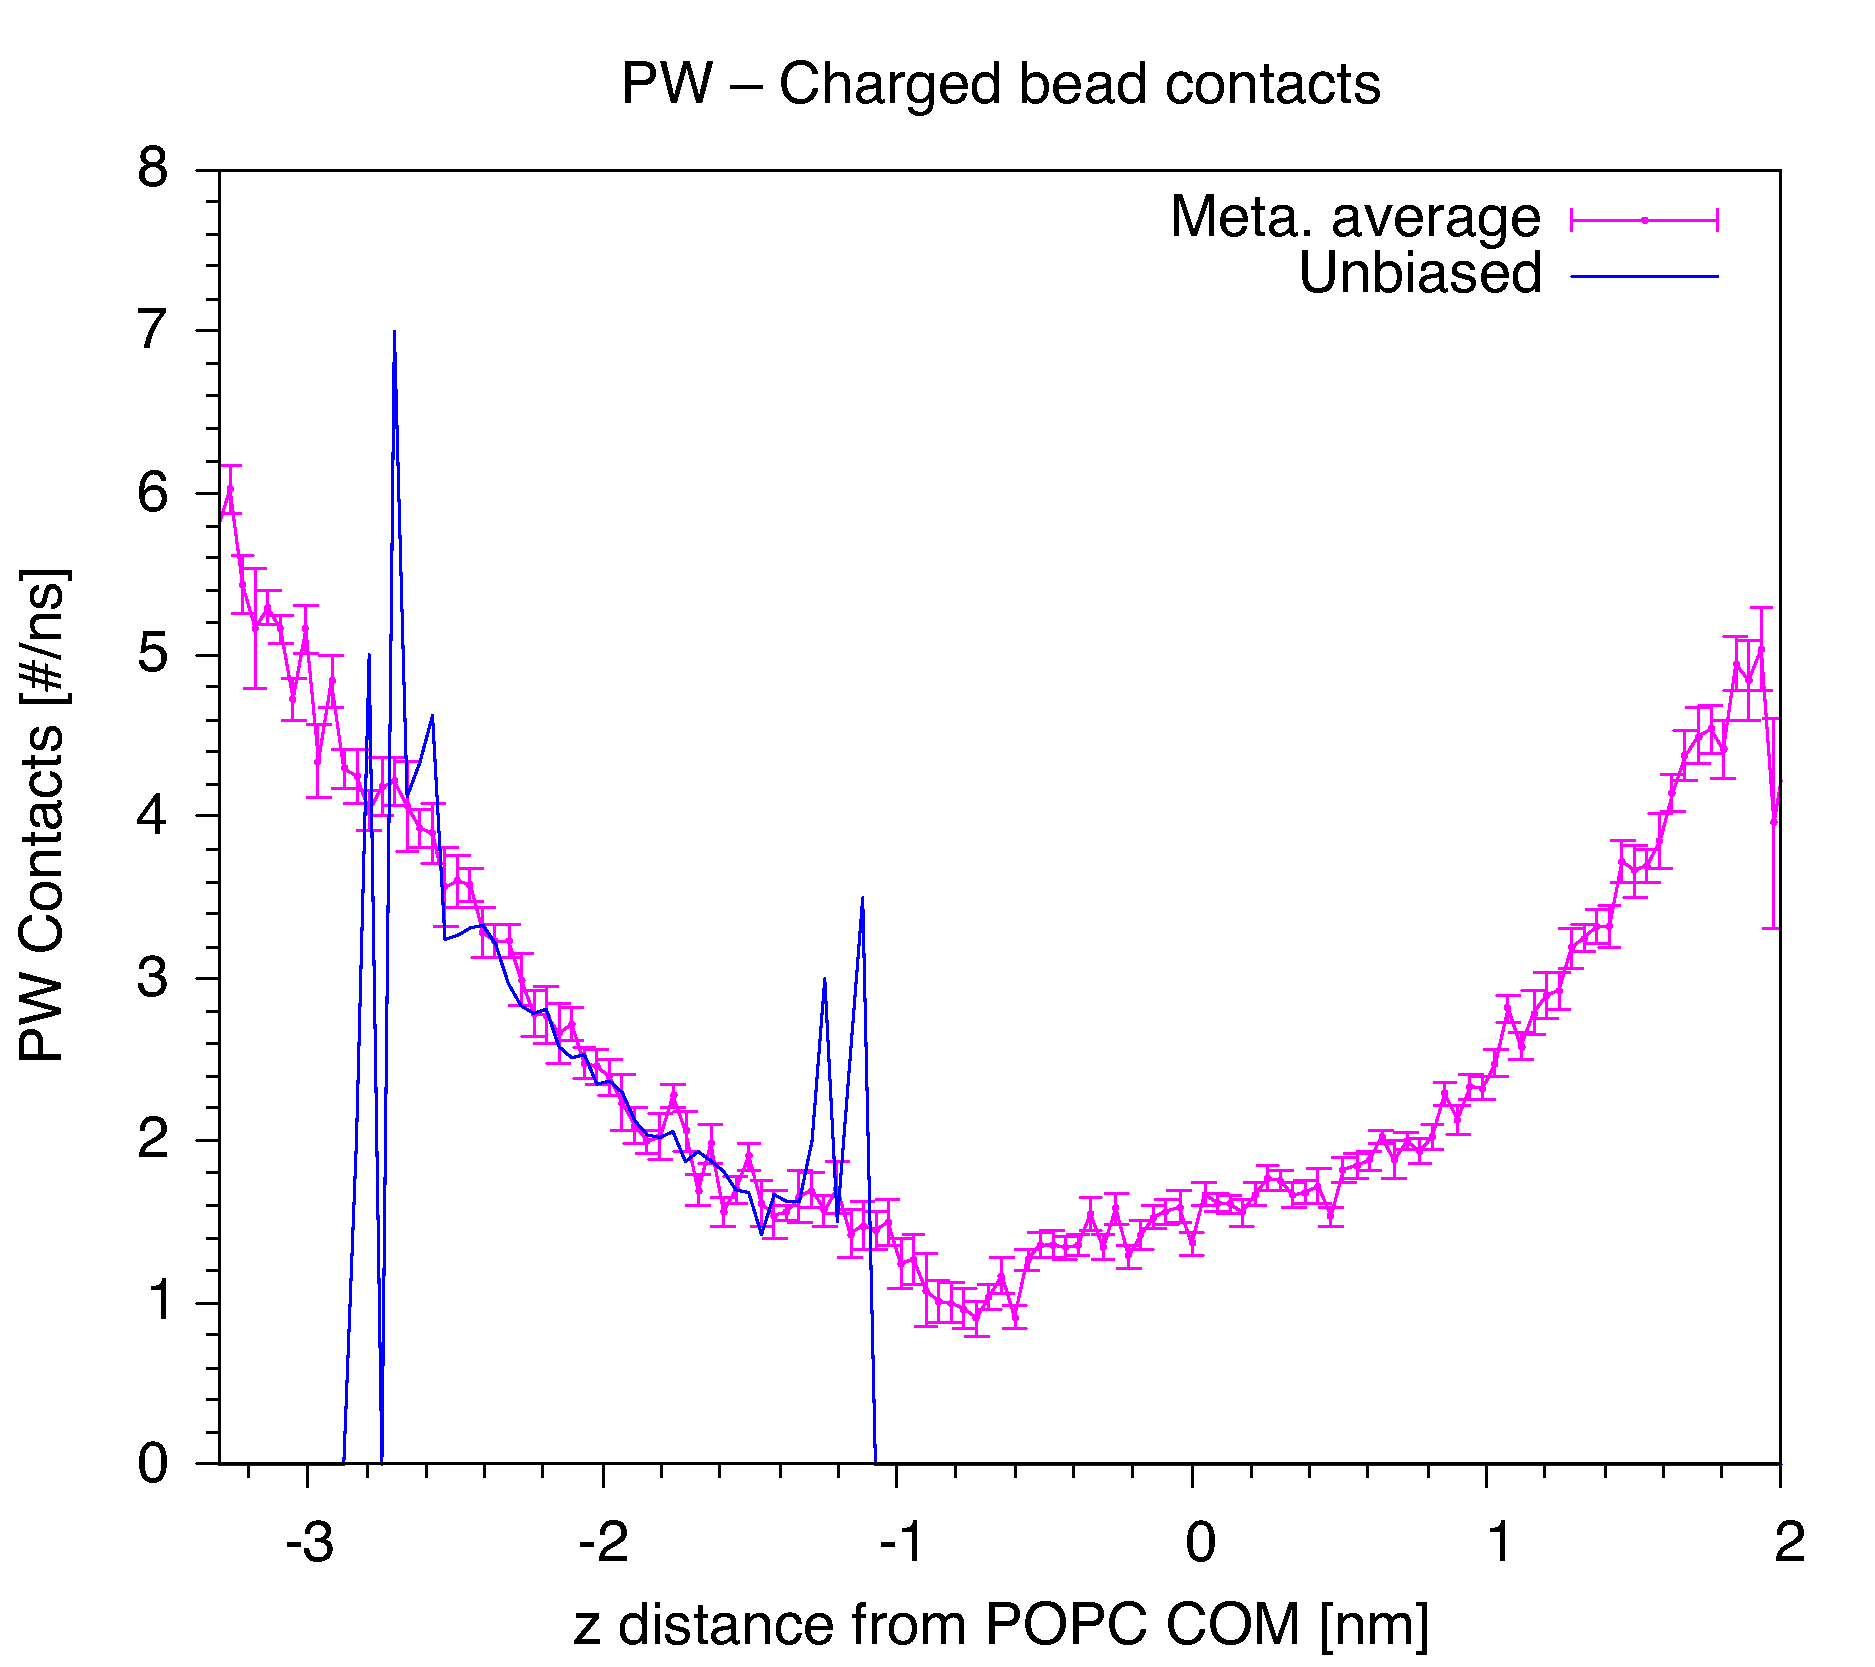
\includegraphics[width=0.5\textwidth]{./img/results/random11PWContact}
	}\\%
	\subfloat[striped NP]{
		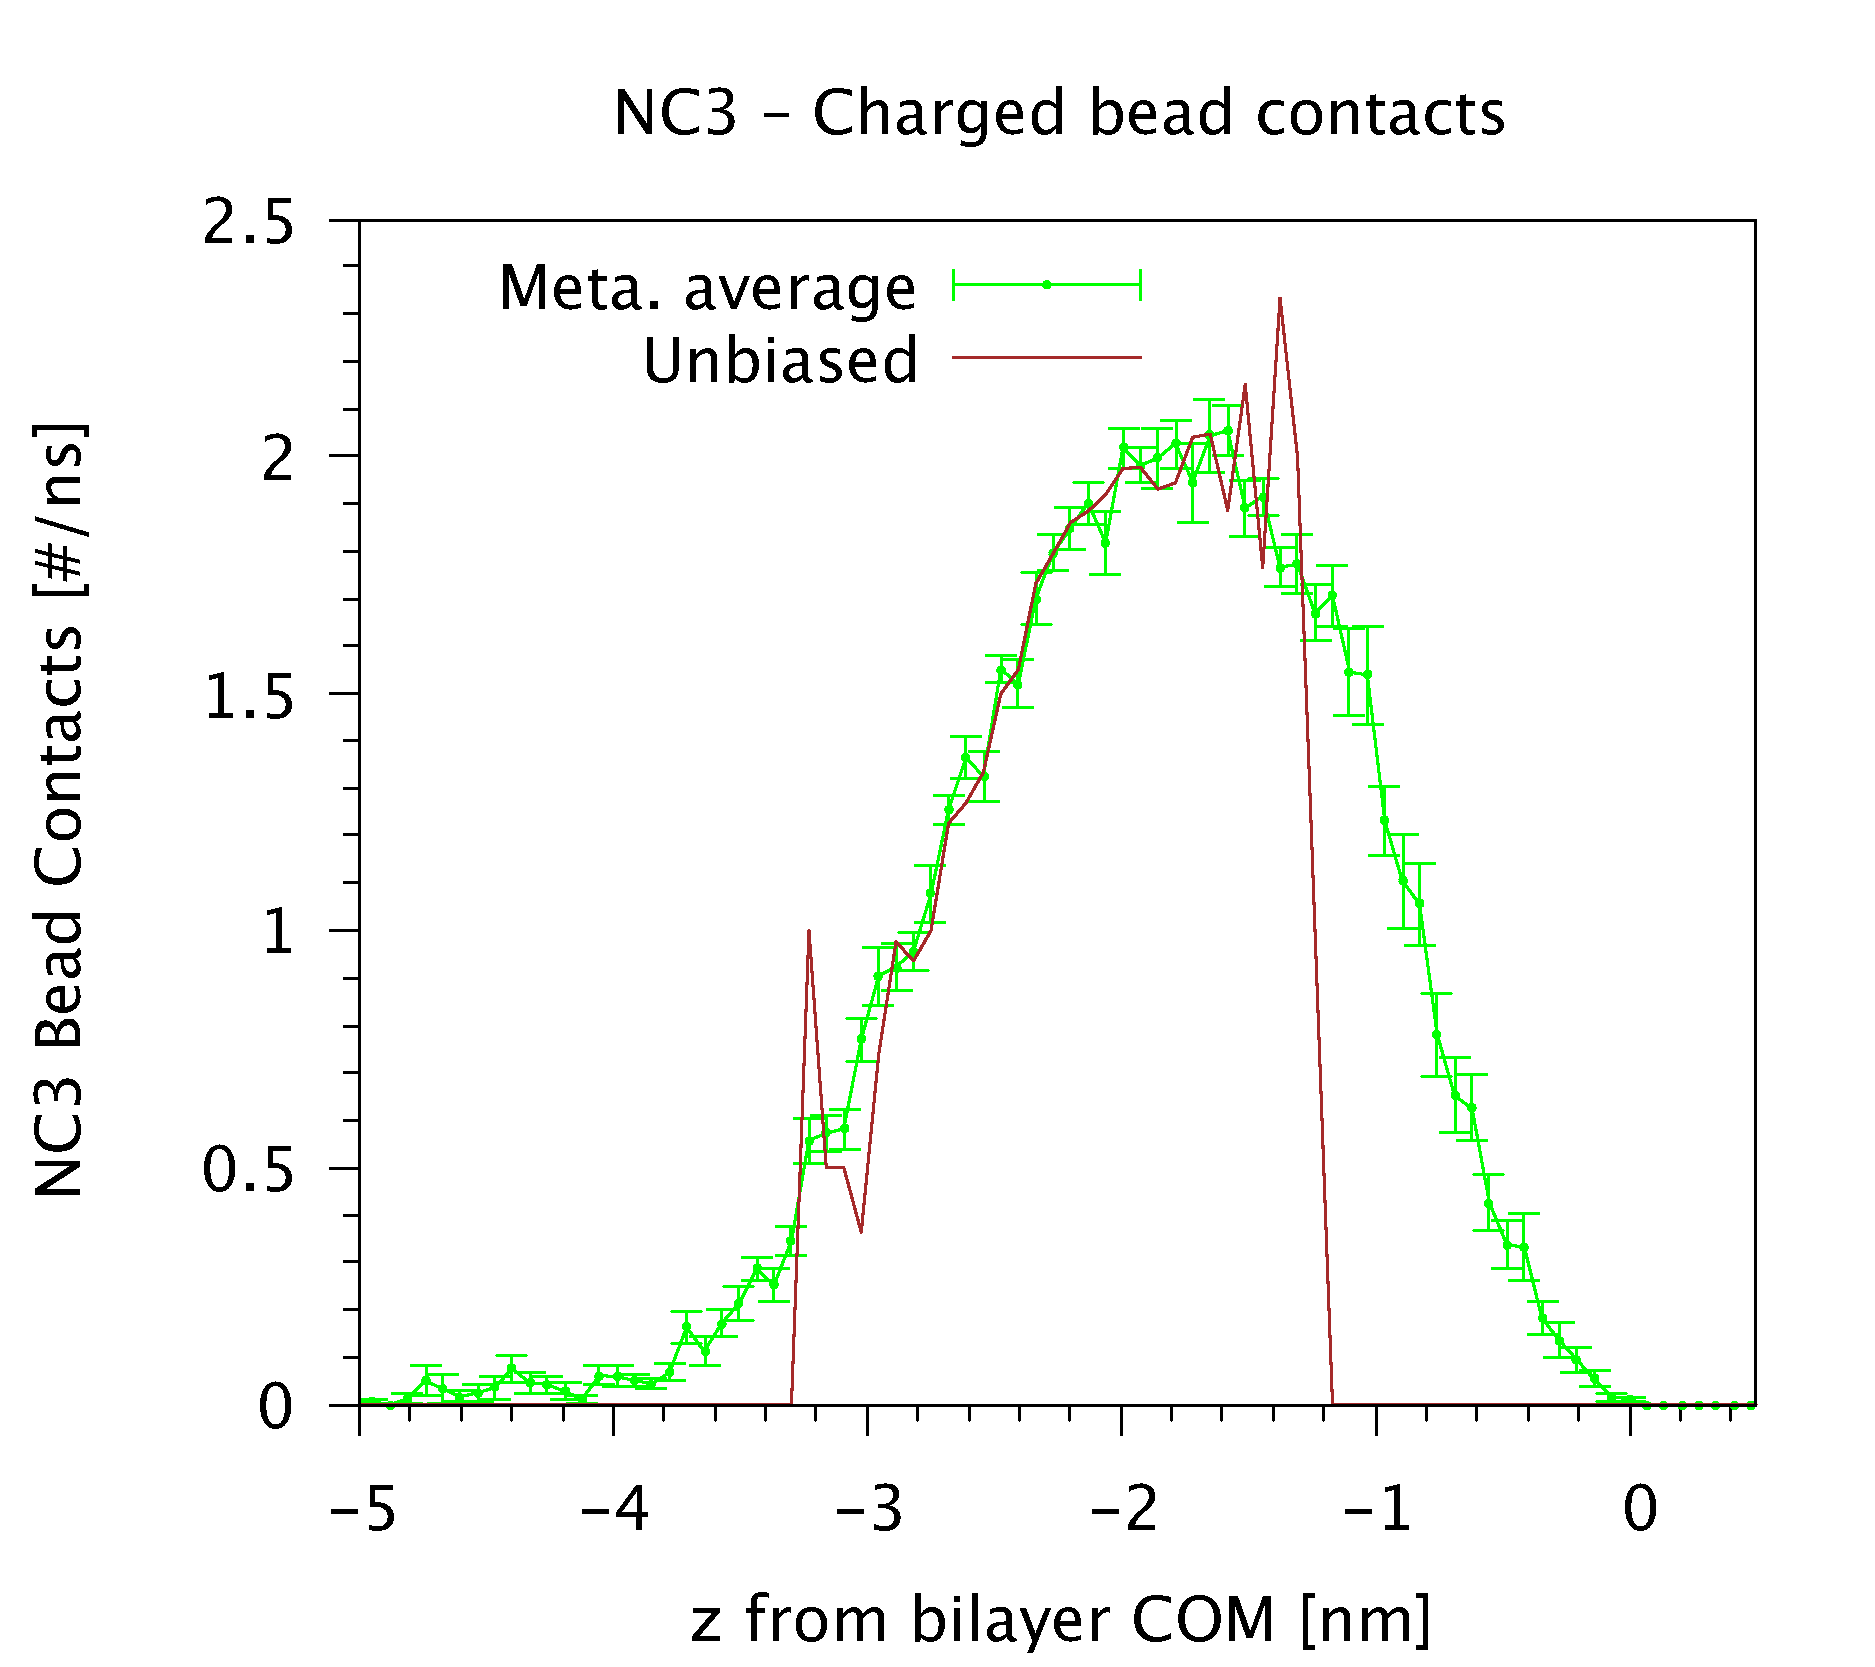
\includegraphics[width=0.5\textwidth]{./img/results/patchedNC3Contact}
	}%
	\subfloat[random NP]{
		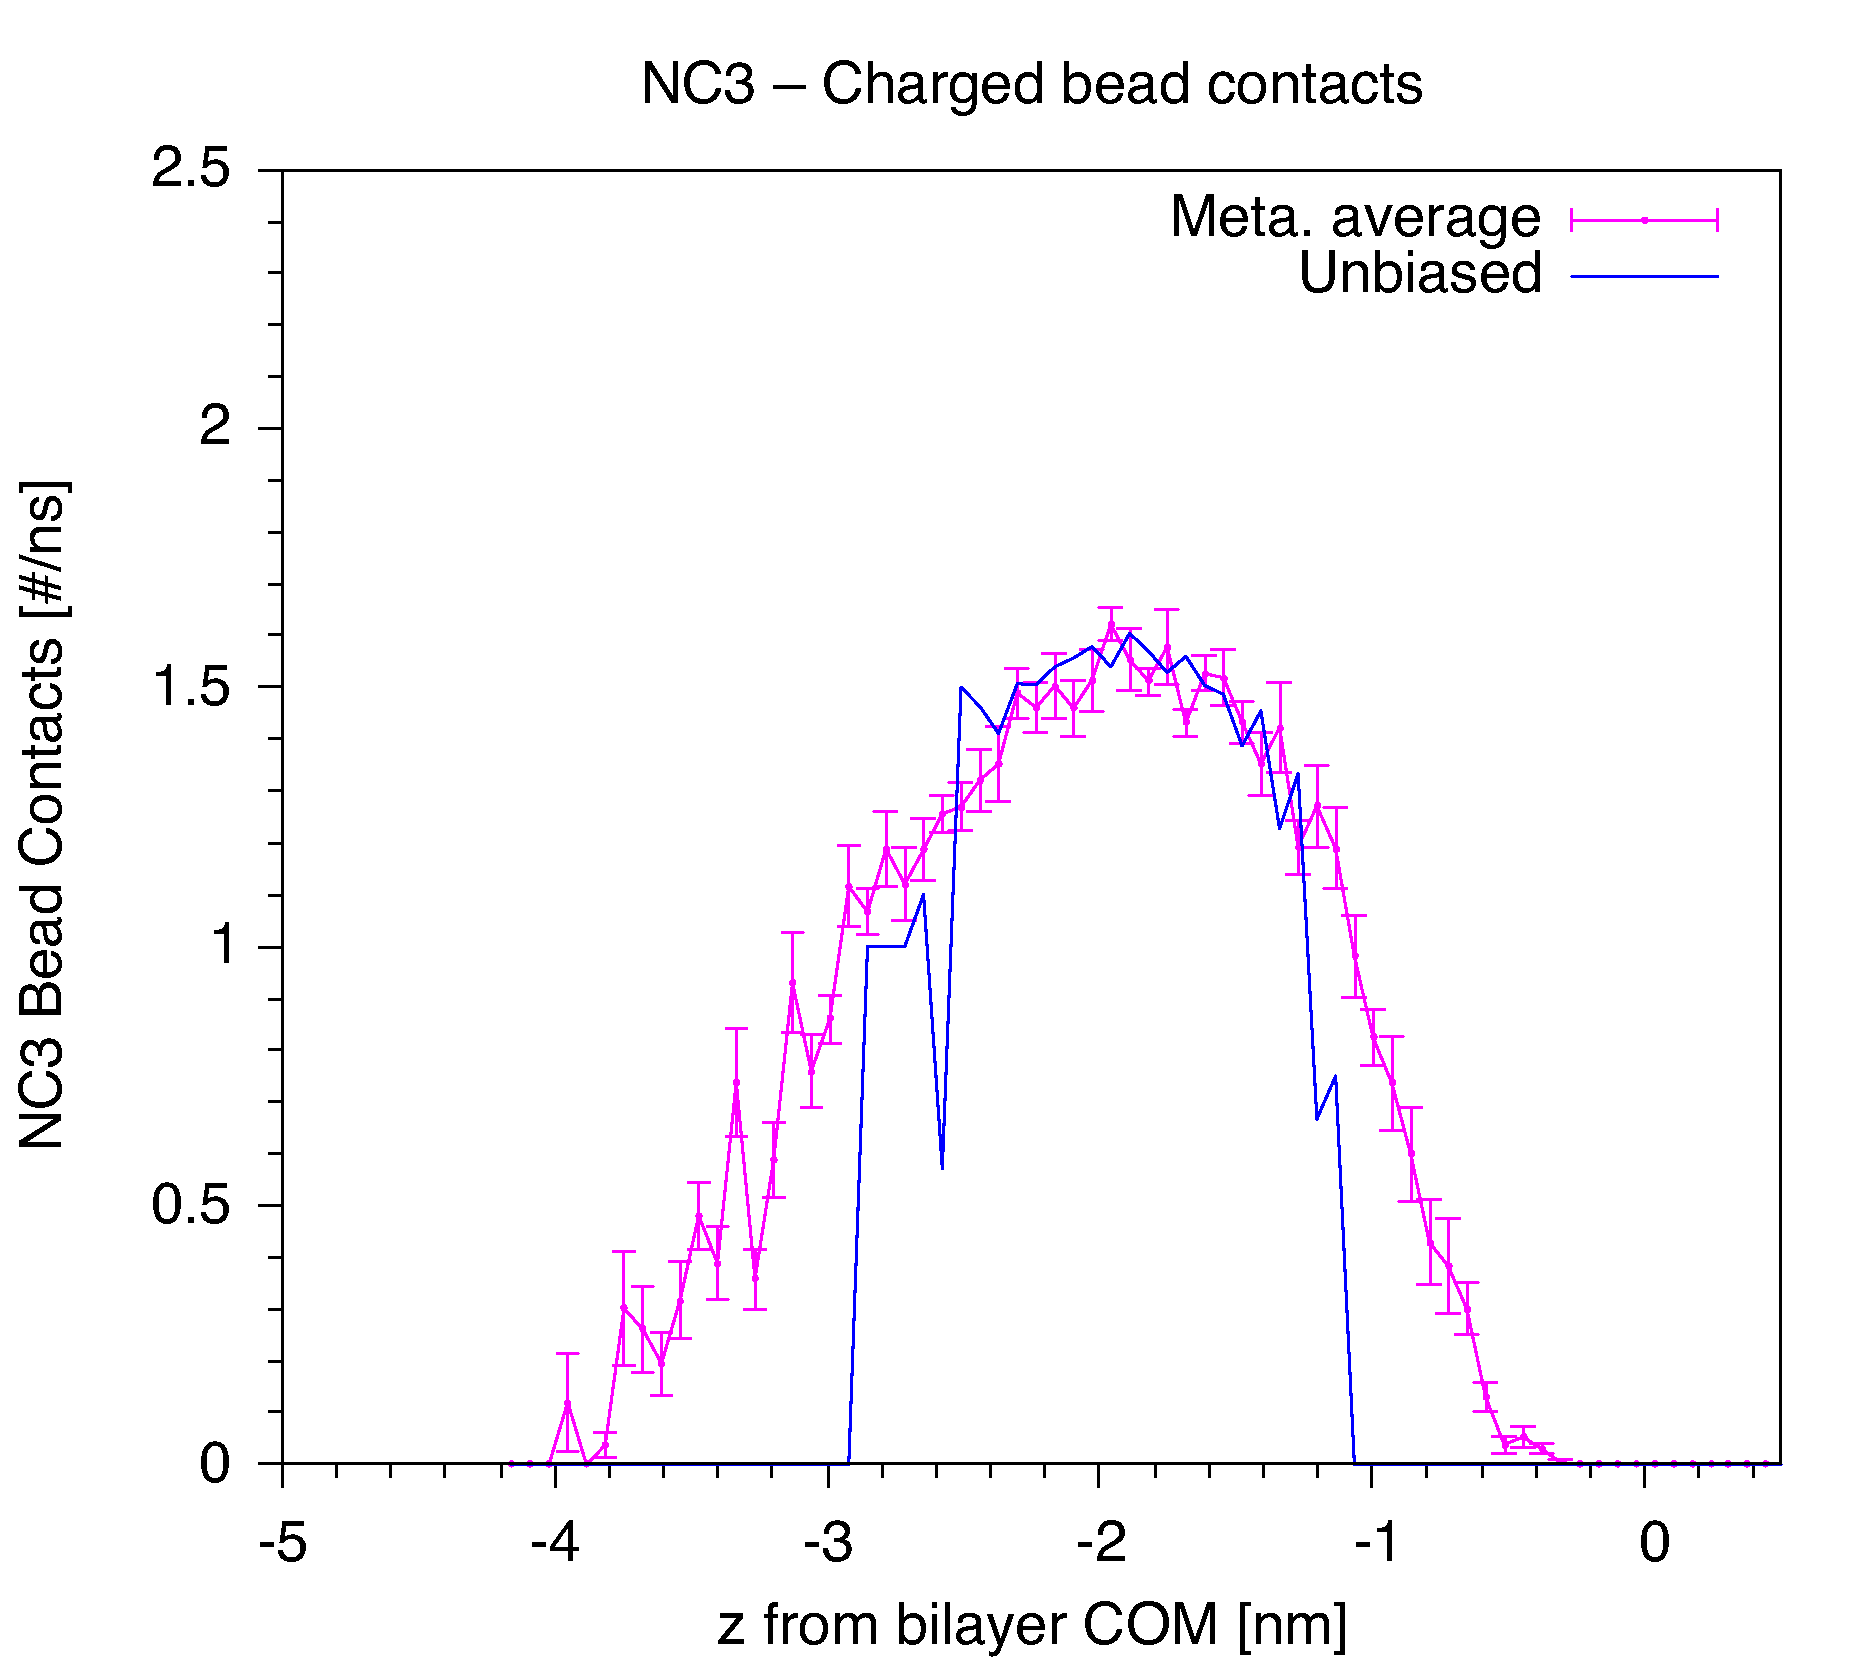
\includegraphics[width=0.5\textwidth]{./img/results/random11NC3Contact}
	}
	\caption{(a-b) Number of contacts per ns between the \acs{PW} beads and the charged bead in function of the position of the charged bead for: (a) the striped \acs{NP} and (b) the random \acs{NP}. (c-d) The same for the coline group and the charged bead  in the hydrophobic state for: (c) the striped \ac{NP} and (d) the random \acs{NP}. For each plots the number of contacts are in comparison with the corresponding unbiased runs.}
\end{figure}
\restoregeometry


\section{NP and membrane properties}
%Proprietà generali
%Coef di diffusione stato ancorato, stato idrofobico

\begin{table}[h!t]
	\centering
	\begin{tabular}{lccc}
		\toprule
		\,		 & striped($1$:$1$)		& random($1$:$1$)		& random($1$:$2$)					\\ \toprule
		$D^h_{\text{NP}}$ [$10^{-8}$~cm$^2$/s] & $12 \pm 2$ & $5 \pm 2$ & $5.7 \pm 0.7$ 				\\ \midrule
		$D_{tl}$ [$10^{-8}$~cm$^2$/s] & $30 \pm 1$ & $\mathbf{25 \pm 1}$ & $\mathbf{27.8 \pm 0.1}$	\\ \midrule
		$D_{bl}$ [$10^{-8}$~cm$^2$/s] & $\mathbf{22 \pm 2}$ & $27 \pm 3$	& $35 \pm 1$			\\ \midrule
		$\overline{d_z}$ [nm] & $1.996 \pm 0.0016$	& $2.2794 \pm 0.0017$	& $2.7284 \pm 0.0014$	\\ \bottomrule
	\end{tabular}
	\caption{Lateral diffusion coefficients: of the \acs{NP} in the hydrophobic state ($D^h_\text{NP}$), of the lipids in the top leaflet ($D_{tl}$) and in the bottom leaflet ($D_{bl}$). $\overline{d_z}$ is the average $z$ component of the distance between the \acs{COM} of the \acs{NP} and the \acs{COM} of the \acs{POPC} bilayer. The values in bold font refer to the entrance leaflet. Data obtained from my unbiased runs.}
	\label{tab:NPMembProperties}
\end{table}


\section{Structural properties of the bilayer}
%Risucchio delle membrane al recrossing
%Deformazione del leaflet di ancoraggio: RDF e densitymap 2D